\section{Numerical experiments}
\label{sec:exp}
%\begin{figure*}[t!]
%	\begin{center}
%		%\vspace{-0em}
%		\setlength{\tabcolsep}{1pt}
%		\begin{tabular}{ccccc}
%			\rotatebox{90}{$~~~~~~~m=4000$} &
%			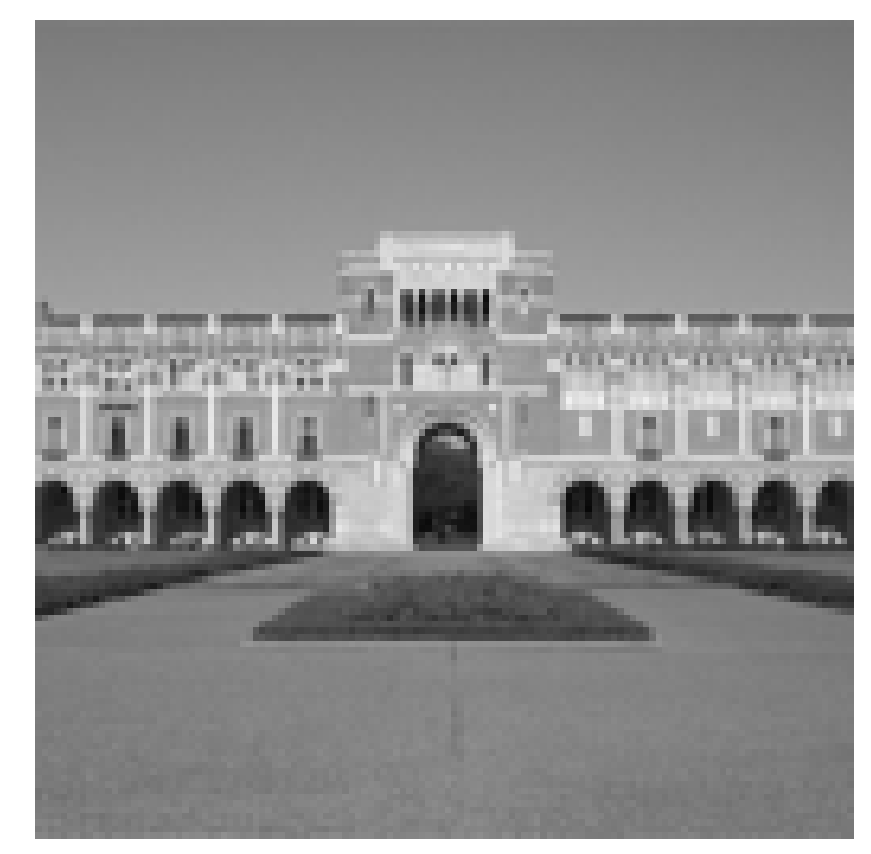
\includegraphics[width=0.22\linewidth]{./fig/lovett_original.pdf} &
%			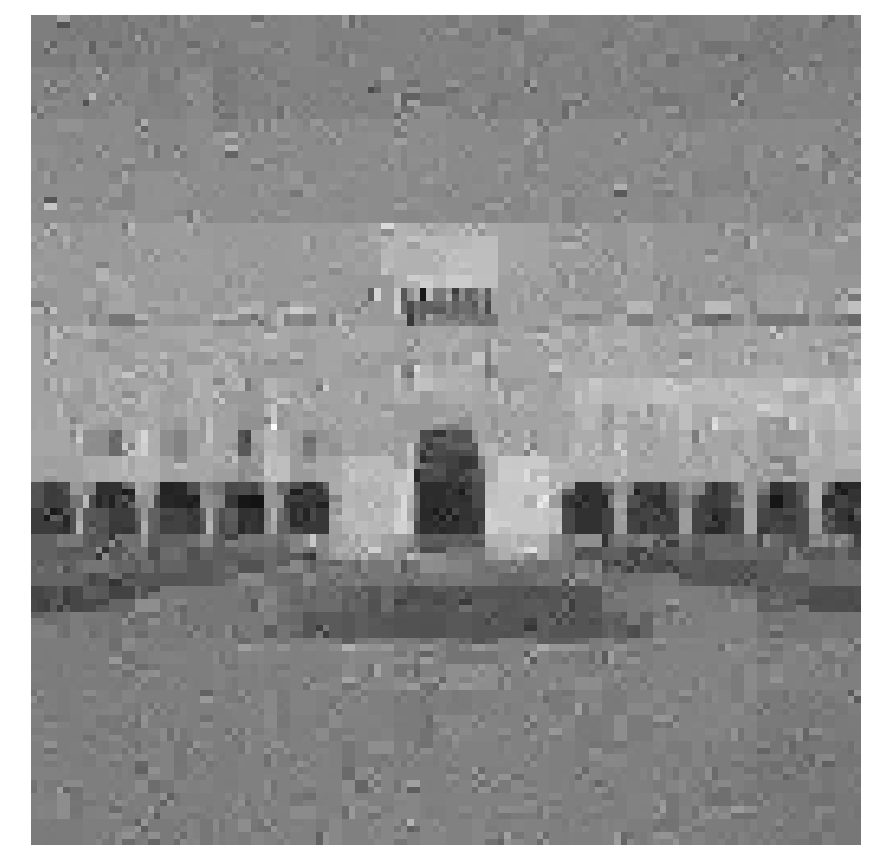
\includegraphics[width=0.22\linewidth]{./fig/lovett_r1_m_4000_s_800.pdf} & 
%			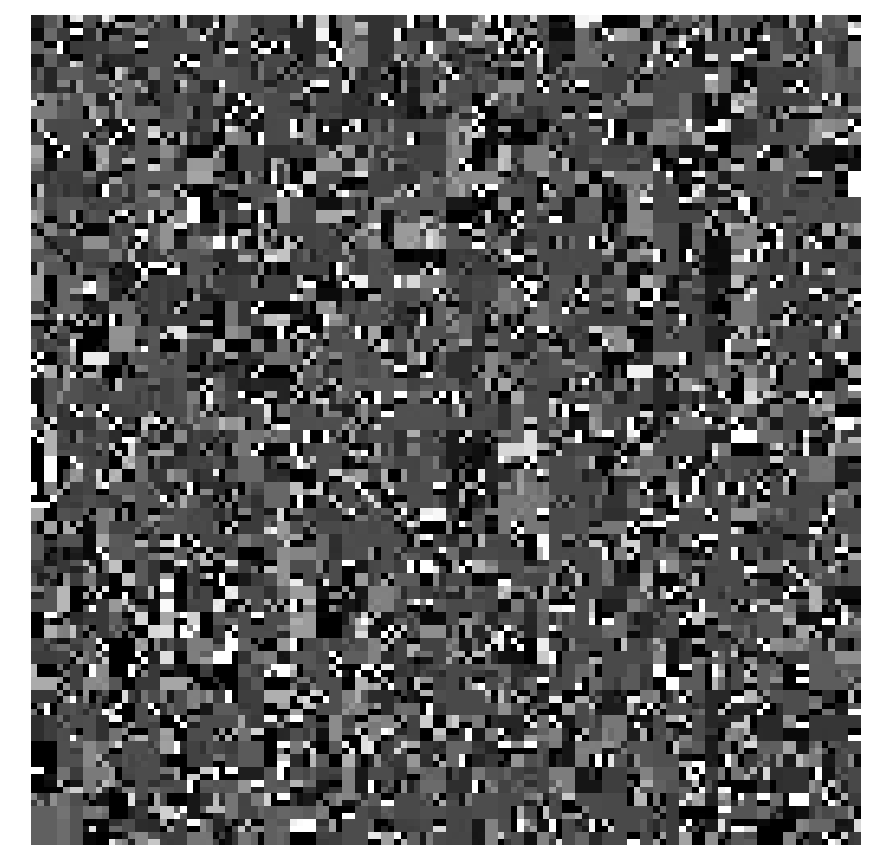
\includegraphics[width=0.22\linewidth]{./fig/lovett_r2_m_4000_s_800.pdf} &
%			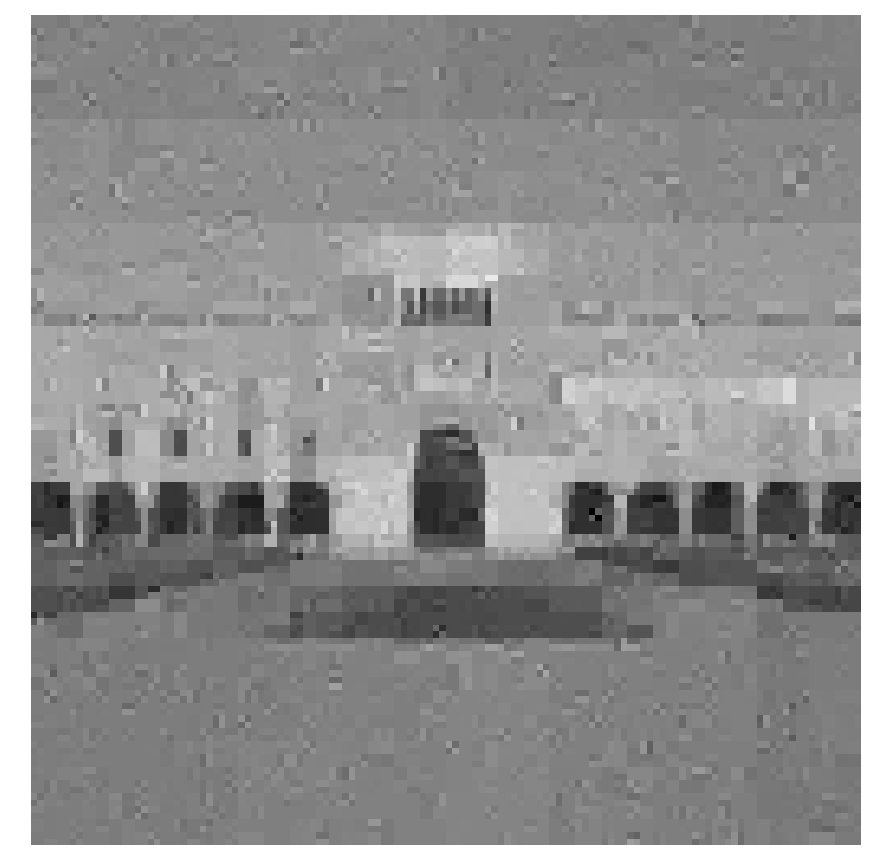
\includegraphics[width=0.22\linewidth]{./fig/lovett_r4_m_4000_s_800.pdf}  \\
%			& \small{(a) Original image}& \small{(b) $R=1$, SNR $=25.06$dB}& \small{(c) $R=2$, SNR $=6.60$dB}& \small{(d) $R=4$, SNR $=26.63$dB} \\
%			
%			\rotatebox{90}{$~~~~~~~m=8000$} &
%			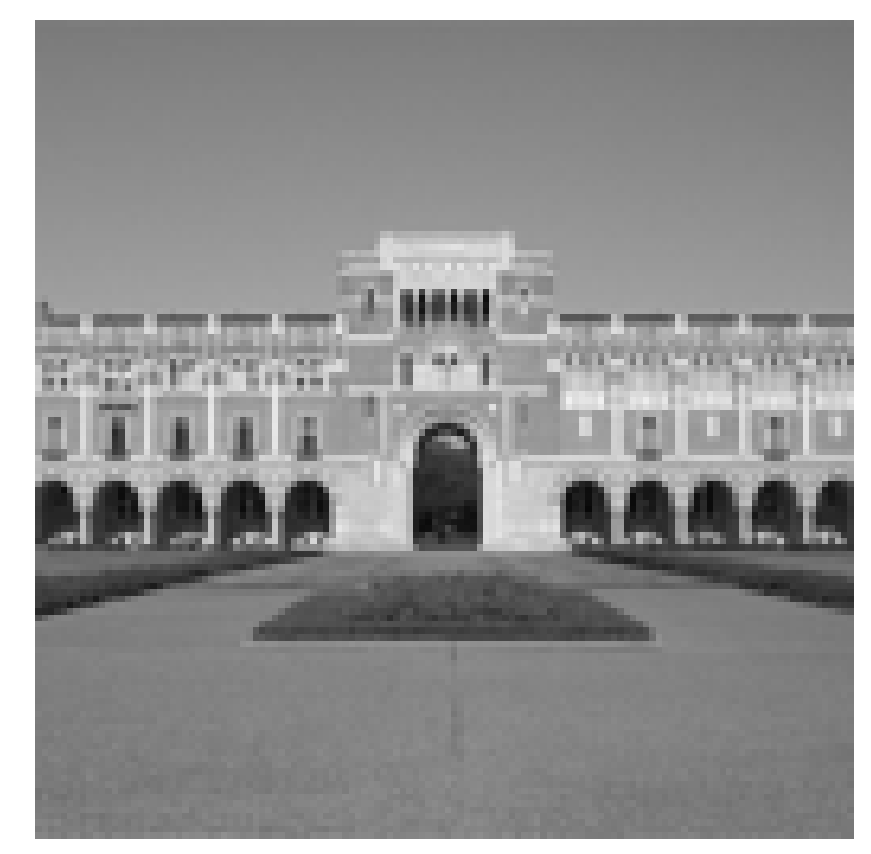
\includegraphics[width=0.22\linewidth]{./fig/lovett_original.pdf} &
%			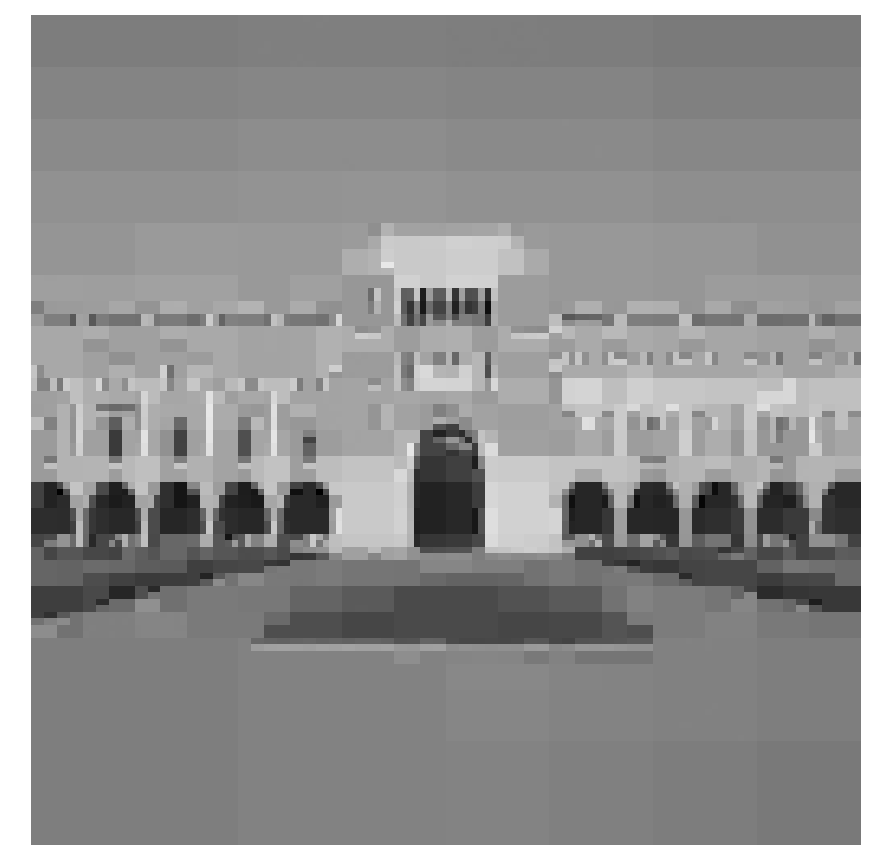
\includegraphics[width=0.22\linewidth]{./fig/lovett_r1_m_8000_s_800.pdf} &
%			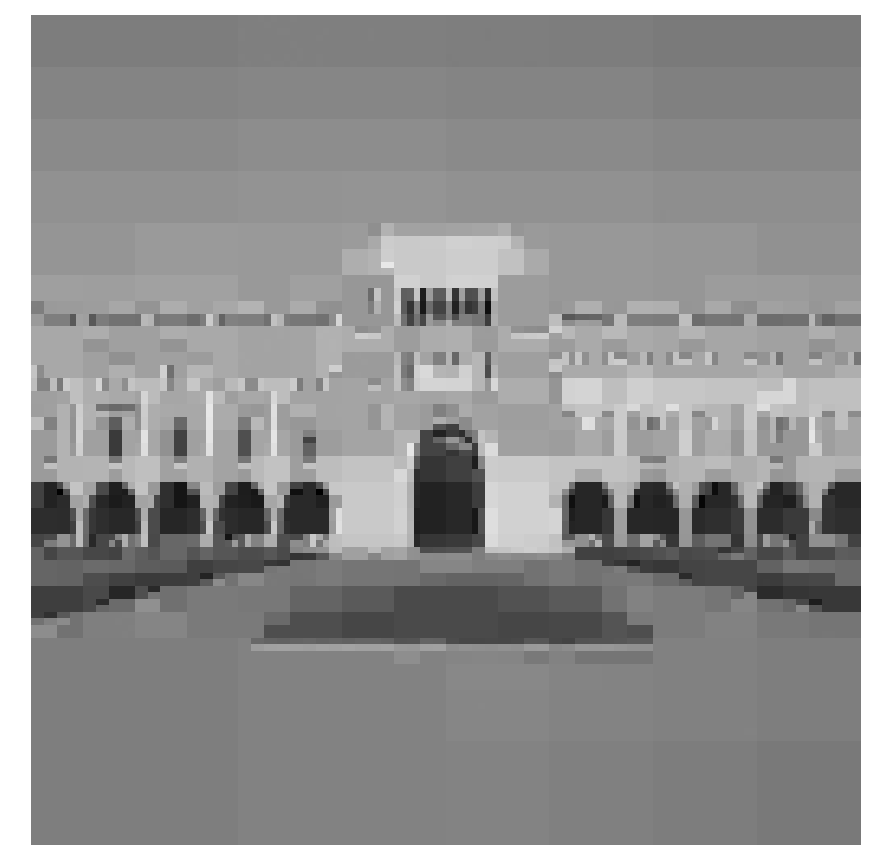
\includegraphics[width=0.22\linewidth]{./fig/lovett_r2_m_8000_s_800.pdf} &
%			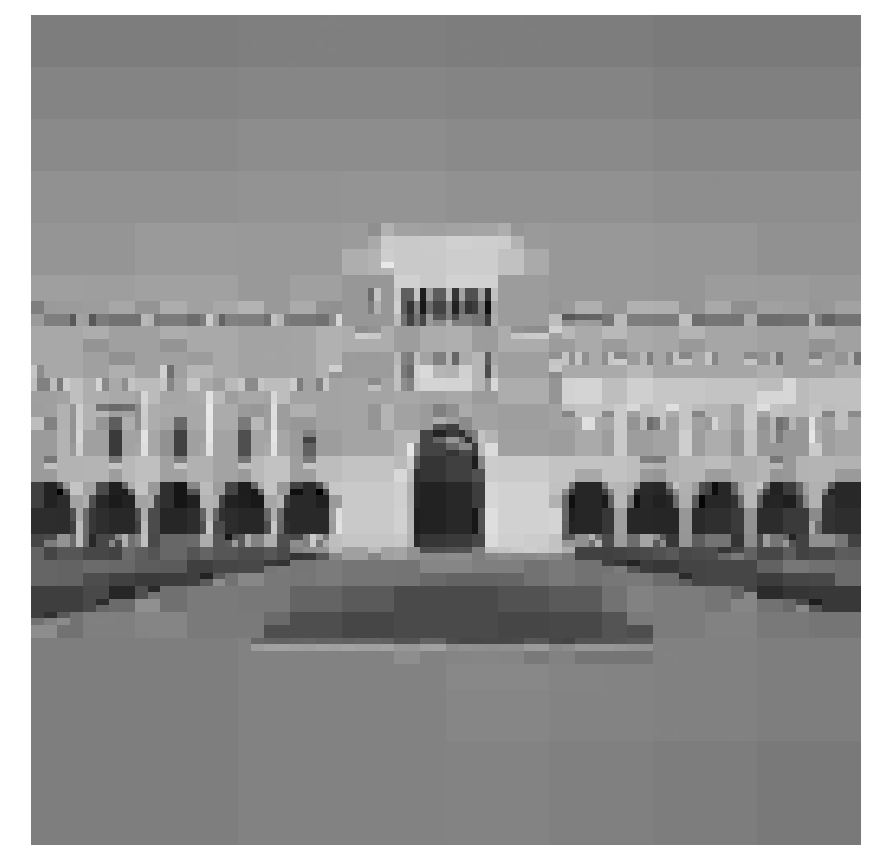
\includegraphics[width=0.22\linewidth]{./fig/lovett_r4_m_8000_s_800.pdf}  \\
%			& \small{(a) Original image}& \small{(b) $R=1$, SNR $=77.71$dB} &\small{ (c) $R=2$, SNR $=76.55$dB} & \small{(d) $R=4$, SNR $=79.29$dB} \\
%		\end{tabular}
%	\end{center}
%	\caption{{(a) Original Lovett Hall image ($n=16,384$); sparse reconstructions ($s=800$) using $m=4000$ (top) and $m=8000$ (bottom) measurements for (b) $R=1$, (c) $R=2$, (d) $R=4$}}
%	\label{fig:lovett}
%\end{figure*}


\begin{figure*}[t!]
	\begin{center}
		%\vspace{-0em}
		\setlength{\tabcolsep}{1pt}
		\begin{tabular}{ccccc}
			\rotatebox{90}{$~~~~~~~m=4000$} &
			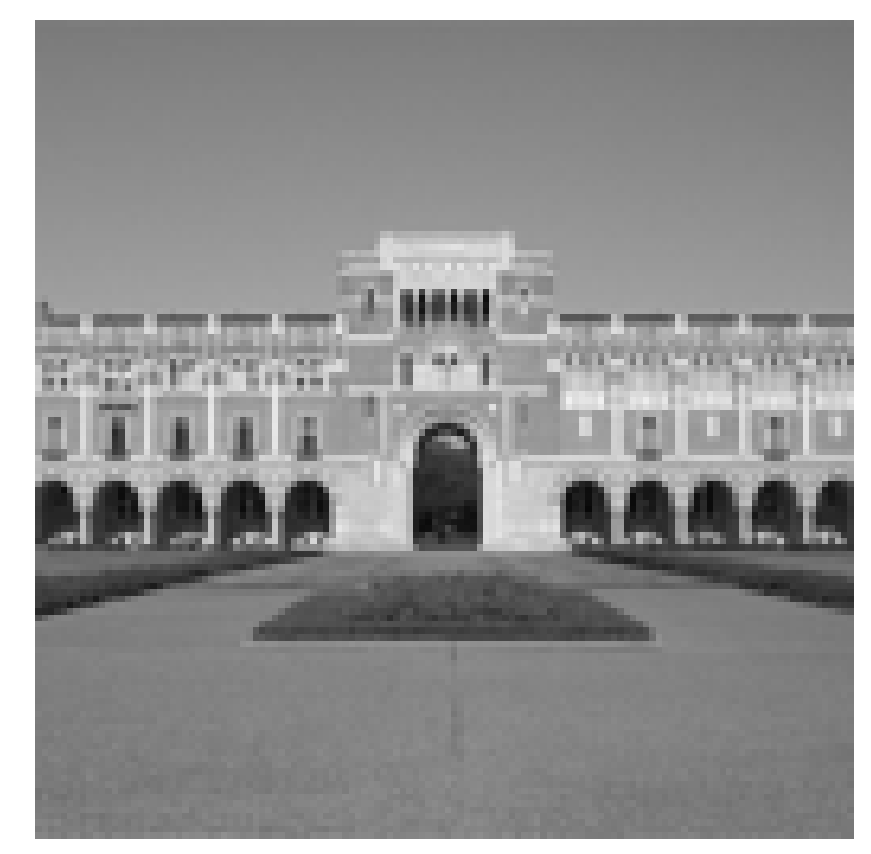
\includegraphics[width=0.22\linewidth]{./fig/lovett_original.pdf} &
			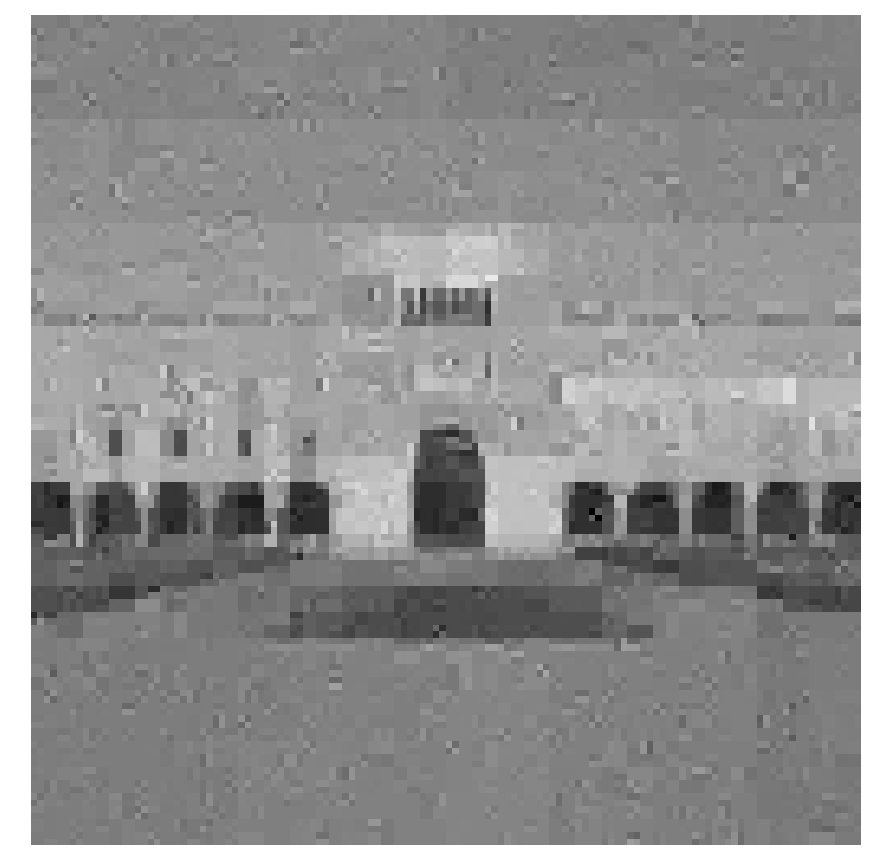
\includegraphics[width=0.22\linewidth]{./fig/lovett_r4_m_4000_s_800.pdf} & 
			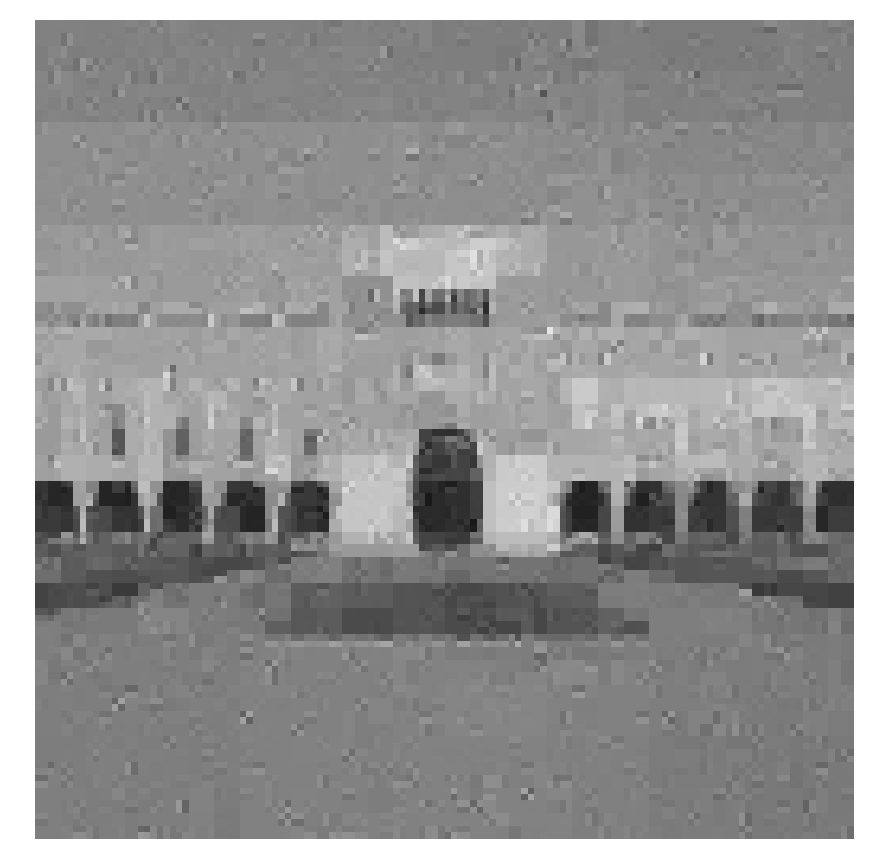
\includegraphics[width=0.22\linewidth]{./fig/lovett_r425_m_4000_s_800.pdf} &
			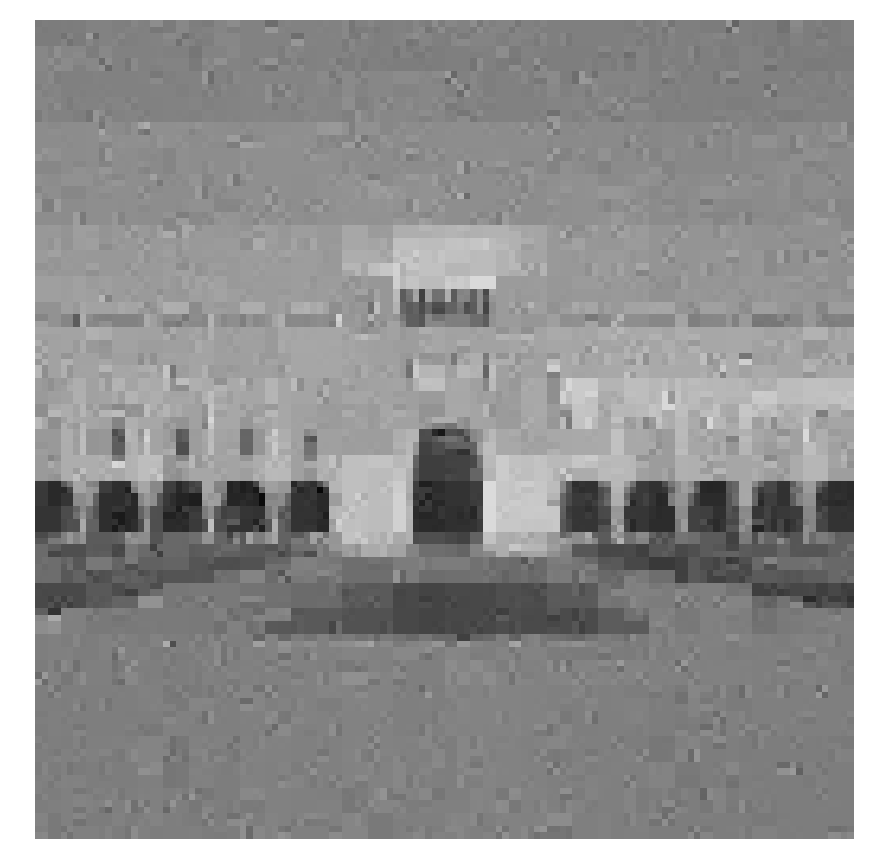
\includegraphics[width=0.22\linewidth]{./fig/lovett_r450_m_4000_s_800.pdf}  \\
			& \small{(a) Original image}& \small{(b) $R=4$, SNR $=26.63$dB}& \small{(c) $R=4.25$, SNR $=27.20$dB}& \small{(d) $R=4.5$, SNR $=27.21$dB} \\
			
			\rotatebox{90}{$~~~~~~~m=6000$} &
			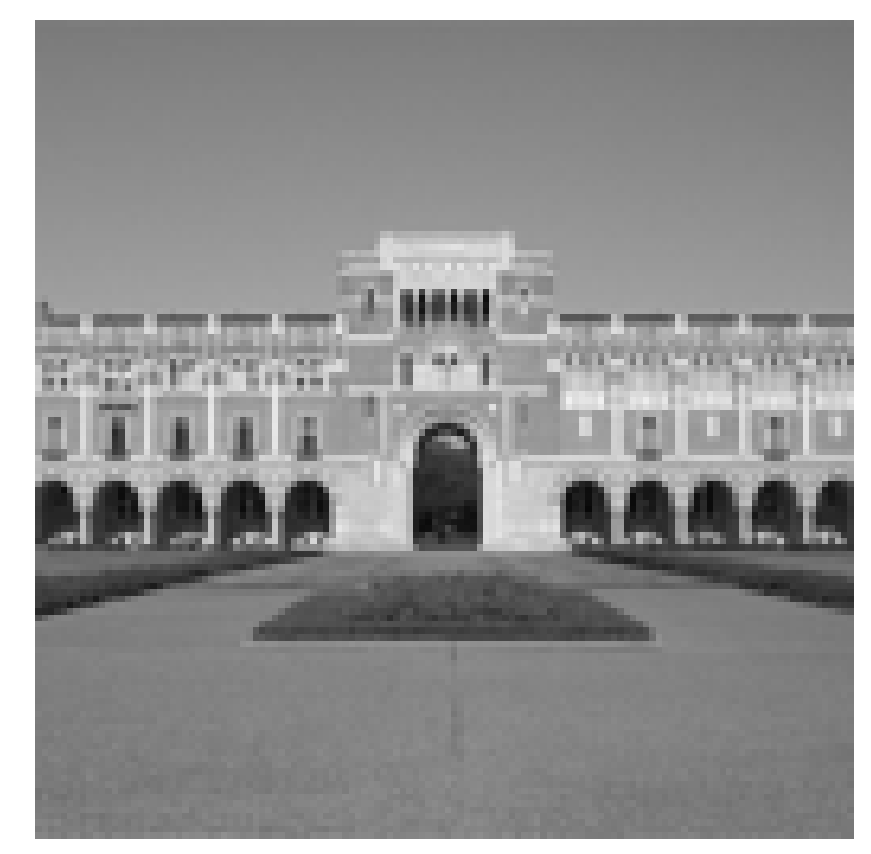
\includegraphics[width=0.22\linewidth]{./fig/lovett_original.pdf} &
			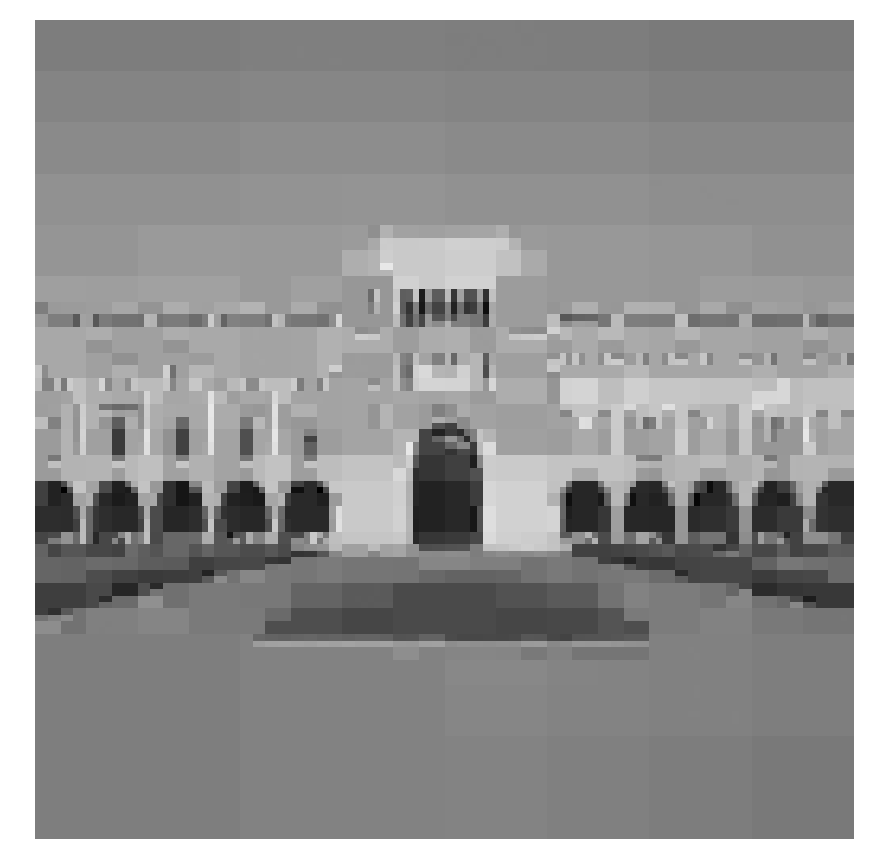
\includegraphics[width=0.22\linewidth]{./fig/lovett_r4_m_6000_s_800.pdf} & 
			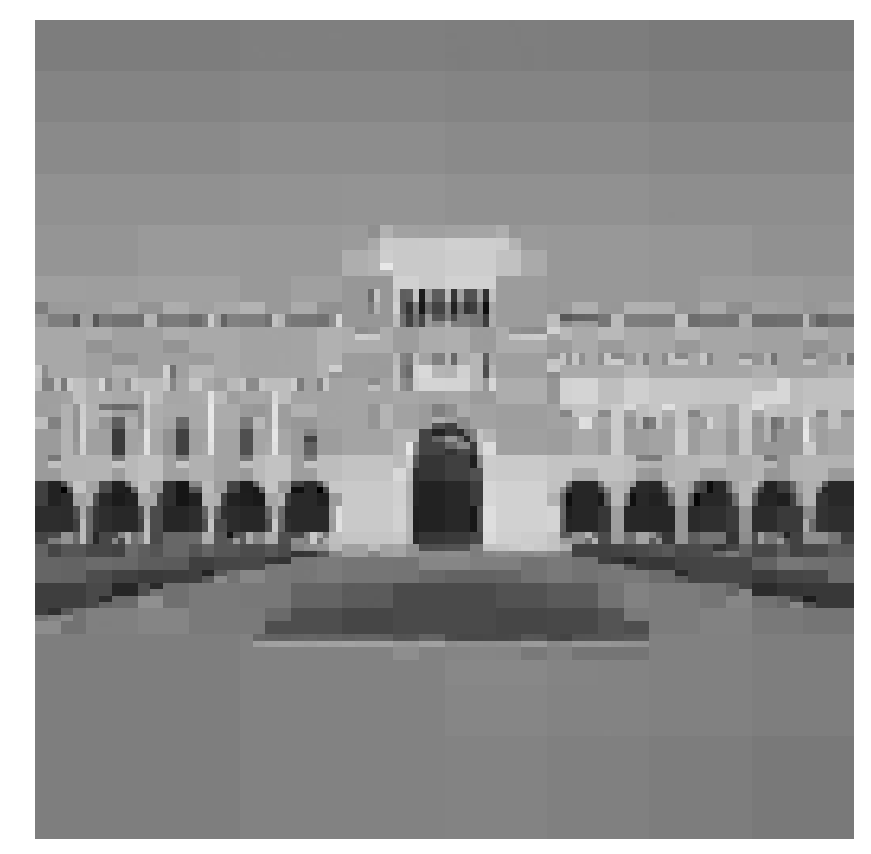
\includegraphics[width=0.22\linewidth]{./fig/lovett_r425_m_6000_s_800.pdf} &
			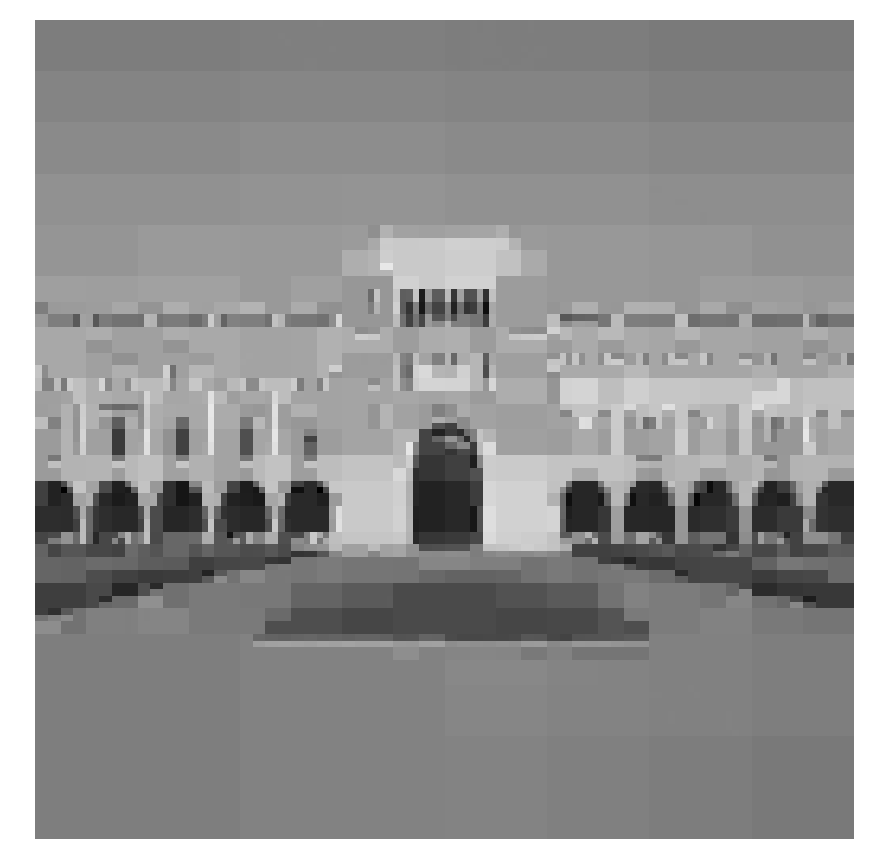
\includegraphics[width=0.22\linewidth]{./fig/lovett_r450_m_6000_s_800.pdf}  \\
			& \small{(a) Original image}& \small{(b) $R=4$, SNR $=81.50$dB}& \small{(c) $R=4.25$, SNR $=82.88$dB}& \small{(d) $R=4.5$, SNR $=83.25$dB} \\
		\end{tabular}
	\end{center}
	\caption{{(a) Original Lovett Hall image ($n=16,384$); sparse reconstructions ($s=800$) using $m=4000$ (top) and $m=6000$ (bottom) measurements for (b) $R=4$, (c) $R=4.25$, (d) $R=4.5$.}}
	\label{fig:lovett}
\end{figure*}

In this section, we present the results of simulations of signal reconstruction using our algorithm. All numerical experiments were conducted using MATLAB R2017a on a Linux system with an Intel CPU and 64GB RAM. Our experiments explores the performance of the MoRAM algorithm on both synthetic data as well as real images.

We perform experiments on a synthetic sparse signal $\mb{x^*} \in \R^n$ with $n=1000$. The sparsity level of the signal is chosen in steps of $3$ starting from $3$ with a maximum value of $12$. The non-zero elements of the test signal $\mb{x^*}$ are generated using zero-mean Gaussian distribution $\mathcal{N}(0, 1)$ and normalized such that $\norm{\mb{x^*}} =1$. The elements of the Gaussian measurement matrix $\mb{A} \in \R^{m\times n}, a_{ij}$ are also generated using the standard normal distribution $\mathcal{N}(0, 1)$. The number of measurements $m$ is varied from $m = 100$ to $m=1000$ in steps of $100$.  

%It is important to note that unlike the absolute value function, the modulo function described in Fig.~\ref{fig:compare}(a) is not scale-invariant. The modulo function works over the quantities $y_{c,i}=\langle \mathbf{a_i} \cdot \mathbf{x^*} \rangle, i=1,..,m$; and it is defined over the parameter $R$; thus depending on the magnitudes of $y_{c,i}$ and $R$ relative to each other, the behavior of the measurement model and the reconstruction algorithm would be altered. For instance, if the value of $R$ is too small compared to the range of the $y_{c,i}$, the modulo operation would hardly have any effect on the measurements, leaving $\mathbf{y_c \approx y}$.

%To enforce the quanti, we fix the signal strength by setting $\norm{\mb{x^*}} =1$ in our experiments, while varying the value of modulo parameter $R$ as ${1,2,4}$.

Using $\mb{A, x^*}$ and $\R$, We first obtain the compressed modulo measurements $\mb{y}$ by passing the signal through forward model described by Eq.~\ref{eq:modmeas2}. We compute the initial estimate $\mathbf{x^0}$ using the algorithm~\ref{alg:RCM}. For reconstruction, algorithm~\ref{alg:MoRAM} is employed. we plot the variation of the relative reconstruction error ($\frac{\norm{\mathbf{x^*-x^T}}}{\norm{\mathbf{x^*}}}$) with number of measurements $m$ for our AltMin based sparse recovery algorithm MoRAM.

For each combination of $R, m$ and $s$, we run $10$ independent Monte Carlo trials, and calculate mean of the relative reconstruction error over these trials. Fig.~\ref{fig:plot} (a), (b) and (c) illustrate the performance of our algorithm for increasing values of $R$ respectively. It is evident that for each combination of $R$ and $s$, our algorithm converges with probability $1$ to give the exact recovery of the true signal (zero relative error) provided enough number of measurements. In all such cases, the minimum number of measurements required for exact recovery are well below the ambient dimension $(n)$ of the underlying signal. 

%Another important factor affecting the reconstruction is the quality of the initial estimate ($\mathbf{{x}^0}$) obtained through first order estimation. As described in~\ref{sec:init}, the quality of the initial estimate is a direct function of number of measurements ($m$). As we set $m$ higher, the initial estimate $\mathbf{{x}^0}$ would move closer to the original signal $\mathbf{{x}^*}$. For our experiments, we consider two ranges of $m$: $m \in [100,1000]$ and $m \in [1000,10000]$.
\subsection{Experiments on real image}
\begin{figure*}[!t]
	\begin{center}
		\begin{tabular}{ccc}
			%\vspace{-0em}
			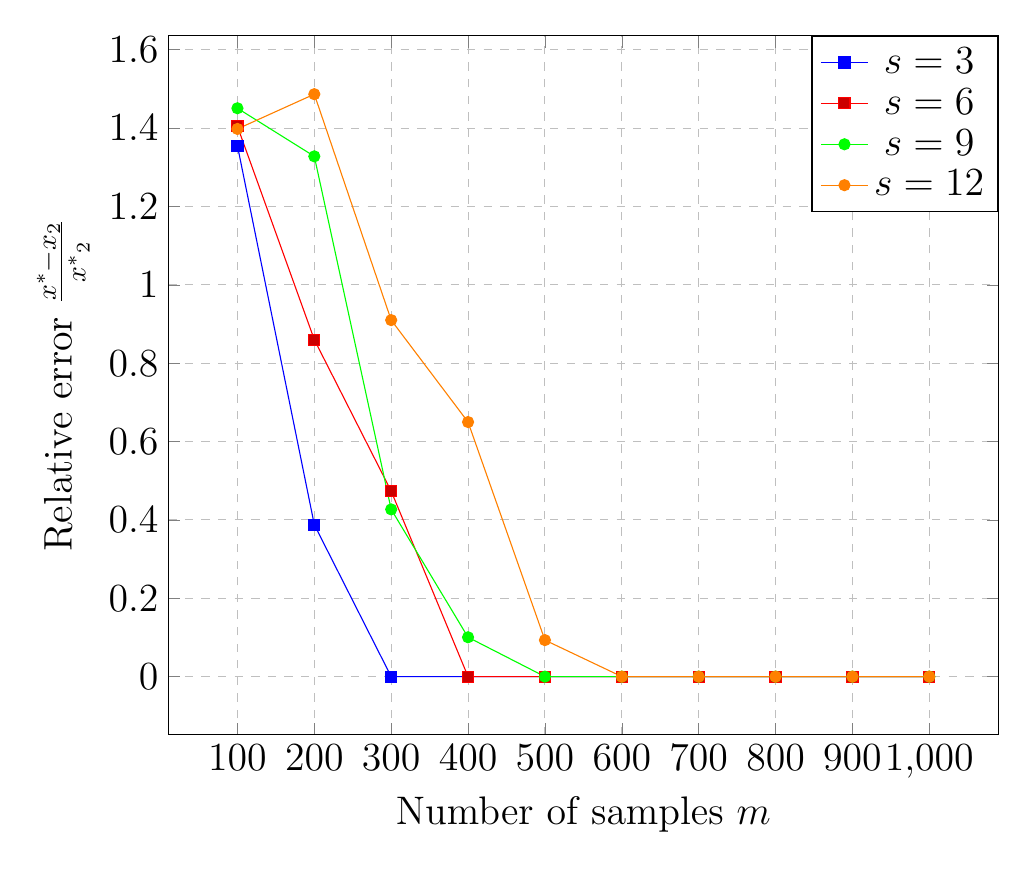
\begin{tikzpicture}
\tikzstyle{every node}=[font=\Large]
\begin{axis}
[width=\linewidth,
xlabel= Number of samples $m$, 
ylabel= Relative error $\frac{\norm{\mb{x^*-x}}_2}{\norm{\mb{x^*}}_2}$,
grid style = dashed,
grid=both,
legend style=
{
at={(1,1), %for arxiv version
%at={(1.65,0.8),  %for NIPS version
anchor=top},
cells={align=center}, 
%legend columns=-1,
} 
]

\addplot[color=blue,mark=square*] plot coordinates {
(100,1.35491249236152)
(200,0.387834861360979)
(300,0.0000838932462760031)
(400,0.0000796709195404289)
(500,0.0000699847485553827)
(600,0.0000654248964096406)
(700,0.0000556622044076941)
(800,0.0000577754338669424)
(900,0.0000476093461140991)
(1000,0.000050430624642886)

};
\addlegendentry{$s=3$};


\addplot plot coordinates {
(100,1.4044226284938)
(200,0.860030446367654)
(300,0.473492899335313)
(400,0.0000833934372627376)
(500,0.0000824008767554939)
(600,0.0000637716674864768)
(700,0.0000644672859553126)
(800,0.0000649831938234799)
(900,0.0000692018122982395)
(1000,0.0000633648746645319)

};

\addlegendentry{$s=6$};


\addplot[color=green,mark=*] plot coordinates {
(100,1.45063072923552)
(200,1.32791017206988)
(300,0.426899433442911)
(400,0.100521404653474)
(500,0.0000847861906819546)
(600,0.0000874052339854557)
(700,0.0000975048393826316)
(800,0.000072296472052776)
(900,0.0000706944130642887)
(1000,0.0000730819848601016)

};
\addlegendentry{$s=9$};

\addplot[color=orange,mark=*] plot coordinates {
(100,1.39786595436235)
(200,1.48655013005159)
(300,0.909955665520478)
(400,0.649802110302209)
(500,0.0932660496014009)
(600,0.0000913091790977068)
(700,0.000104507094662964)
(800,0.0000965628384101342)
(900,0.0000934605996504098)
(1000,0.0000841210242777489)	
};
\addlegendentry{$s=12$};



%\legend{CoPRAM\\Block CoPRAM\\ThWF\\SPARTA\\}

\end{axis}
\end{tikzpicture}
			&
			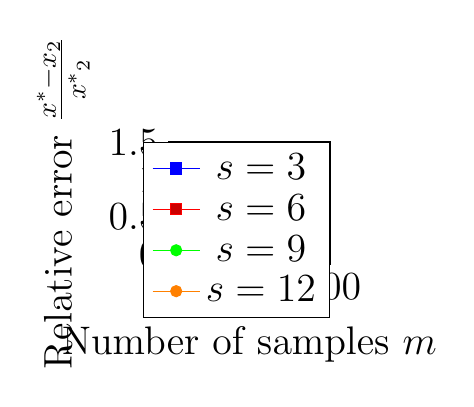
\begin{tikzpicture}
\begin{axis}
[width=0.3\textwidth,
xlabel= Number of samples $m$, 
ylabel= Relative error $\frac{\norm{\mb{x^*-x}}_2}{\norm{\mb{x^*}}_2}$,
grid style = dashed,
grid=both,
legend style=
{
at={(1,1), %for arxiv version
%at={(1.65,0.8),  %for NIPS version
anchor=top},
cells={align=center}, 
%legend columns=-1,
} 
]

\addplot[color=blue,mark=square*] plot coordinates {
	(100,0.747375723427608)
	(200,0.155095058698698)
	(300,0.0000819832015109237)
	(400,0.0000795274009640216)
	(500,0.0000641794969526483)
	(600,0.0000695356190000224)
	(700,0.0000613755178216418)
	(800,0.000066926164718668)
	(900,0.0000621778223230091)
	(1000,0.0000567630039894841)
};
\addlegendentry{$s=3$};


\addplot plot coordinates {
(100,1.27659964262396)
(200,0.43032378497965)
(300,0.0000910097212427942)
(400,0.0000954106153959511)
(500,0.0000809830346078354)
(600,0.0000657018308358537)
(700,0.0000812049368096766)
(800,0.0000603853227824464)
(900,0.000061849877746736)
(1000,0.0000623366305719791)
};

\addlegendentry{$s=6$};


\addplot[color=green,mark=*] plot coordinates {
(100,1.33360297687866)
(200,0.695654696202488)
(300,0.379473134000177)
(400,0.000102603470161568)
(500,0.000103129235494395)
(600,0.0000859751501828087)
(700,0.0000828224635500562)
(800,0.0000879068415403419)
(900,0.0000671510294321006)
(1000,0.0000630635849783938)
};
\addlegendentry{$s=9$};

\addplot[color=orange,mark=*] plot coordinates {
(100,1.36704835741717)
(200,0.932318539564495)
(300,0.559981038525355)
(400,0.000119464801989713)
(500,0.000091109865406022)
(600,0.0000977493433158512)
(700,0.000114550943002834)
(800,0.0000954985216580123)
(900,0.0000848854981296593)
(1000,0.0000637656776977681)
};
\addlegendentry{$s=12$};



%\legend{CoPRAM\\Block CoPRAM\\ThWF\\SPARTA\\}

\end{axis}
\end{tikzpicture}
			&
			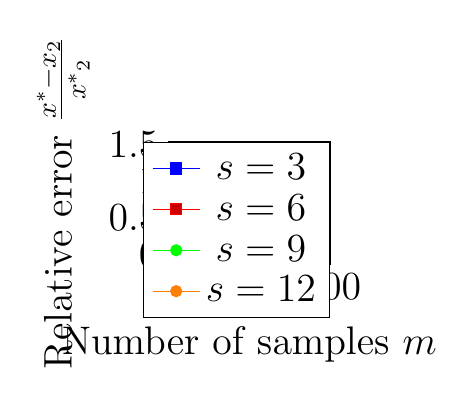
\begin{tikzpicture}
\begin{axis}
[width=0.30\textwidth,
xlabel= Number of samples $m$, 
ylabel= Relative error $\frac{\norm{\mb{x^*-x}}_2}{\norm{\mb{x^*}}_2}$,
grid style = dashed,
grid=both,
legend style=
{
	at={(1,1), %for arxiv version
		%at={(1.65,0.8),  %for NIPS version
		anchor=top},
	cells={align=center}, 
	%legend columns=-1,
} 
]

\addplot[color=blue,mark=square*] plot coordinates {
(100,0.577929457493856)
(200,0.0000837291793747255)
(300,0.0000793871859744244)
(400,0.0000727181866723273)
(500,0.0000754214852024106)
(600,0.0000687961736114565)
(700,0.0000623167482713836)
(800,0.0000630567013152093)
(900,0.0000697408174143524)
(1000,0.0000543869459810252)	
};
\addlegendentry{$s=3$};


\addplot plot coordinates {
	(100,1.08055357197184)
	(200,0.142372501130515)
	(300,0.0000935564761004083)
	(400,0.0000795128007625932)
	(500,0.0000766601332448082)
	(600,0.0000845035092595471)
	(700,0.0000683627818824363)
	(800,0.000054690127278032)
	(900,0.000046380940393624)
	(1000,0.0000628554892293739)
};

\addlegendentry{$s=6$};


\addplot[color=green,mark=*] plot coordinates {
	(100,1.15918634874218)
	(200,0.405732695159951)
	(300,0.0000914377553223125)
	(400,0.0000883373156450208)
	(500,0.0000851861043555281)
	(600,0.000104493988312921)
	(700,0.0000757840403924851)
	(800,0.000070472617739003)
	(900,0.0000882740750443083)
	(1000,0.0000598602984696781)
};
\addlegendentry{$s=9$};

\addplot[color=orange,mark=*] plot coordinates {
	(100,1.39131288865929)
	(200,0.730994731611156)
	(300,0.000118809023021691)
	(400,0.000115250288948783)
	(500,0.0000746863107317379)
	(600,0.00007554657890004)
	(700,0.0000865141368739436)
	(800,0.0000894271050137344)
	(900,0.000076219443854958)
	(1000,0.0000749779527497512)
};
\addlegendentry{$s=12$};



%\legend{CoPRAM\\Block CoPRAM\\ThWF\\SPARTA\\}

\end{axis}
\end{tikzpicture} \\
			(a) & (b) & (c) \\
			%\begin{figure}[t]
			%	\begin{center}
			%\vspace{-0em}	
		\end{tabular}
	\end{center}
	\caption{{Mean relative reconstruction error vs no. of measurements $(m)$ for MoRAM with $\norm{\mb{x^*}}_2=1,n=1000$, and (a) $R=4$; (b) $R=4.25$; (c) $R=4.5$.}}
	\label{fig:plot}
\end{figure*}

We also evaluated the performance of our algorithm on a real image. We obtain sparse representation of the real image by transforming the original image in the wavelet basis (db1). The image used in our experiment is $128 \times 128$ ($n=16384$) image of Lovett Hall (fig.~\ref{fig:lovett}(a)), and  we use the thresholded wavelet transform (with Haar wavelet) to sparsify this image with $s = 800$. We reconstruct the image with MoRAM using $m = 4000$ and $m=6000$ compressed modulo measurements, for $3$ different values of $R$, $4,4.25$ and $4.5$. As expected, the reconstruction performance increases with increasing value of $R$. As shown in Fig.~\ref{fig:lovett}(bottom), for $m=6000$, The algorithm produces near-perfect recovery for all $3$ values of $R$ with high PSNR.
%
%\begin{center}
%	\begin{table}[h]
%		\centering
%		\begin{tabular}{ccc}\toprule
%			\multicolumn{3}{c}{\small{\textbf{Fixed:} $n=1000,\norm{\mathbf{{x}^*}}=1$}} \\ \midrule
%			\multicolumn{3}{c}{\textbf{Justice Pursuit}}
%			\\\cmidrule(r){1-3}%\cmidrule(r){3-4}  
%			\small{$R =1$}&\small{$R=2$}&\small{$R=4$} \\\midrule
%			\hyperref[fig:plot-2-1]{Figure~\ref{fig:plot-2-1}} & \hyperref[fig:plot-2-2]{Figure~\ref{fig:plot-2-2}}
%			& \hyperref[fig:plot-2-3]{Figure~\ref{fig:plot-2-3}} \\
%			\bottomrule
%		\end{tabular}
%		\caption{The Results}\label{Tab3}
%	\end{table} 	
%\end{center}
%In the Table~\ref{Tab3}, we provide experimental results for each of the combination above.

%\begin{figure}[h]
%	\begin{center}
%		%\vspace{-0em}
%		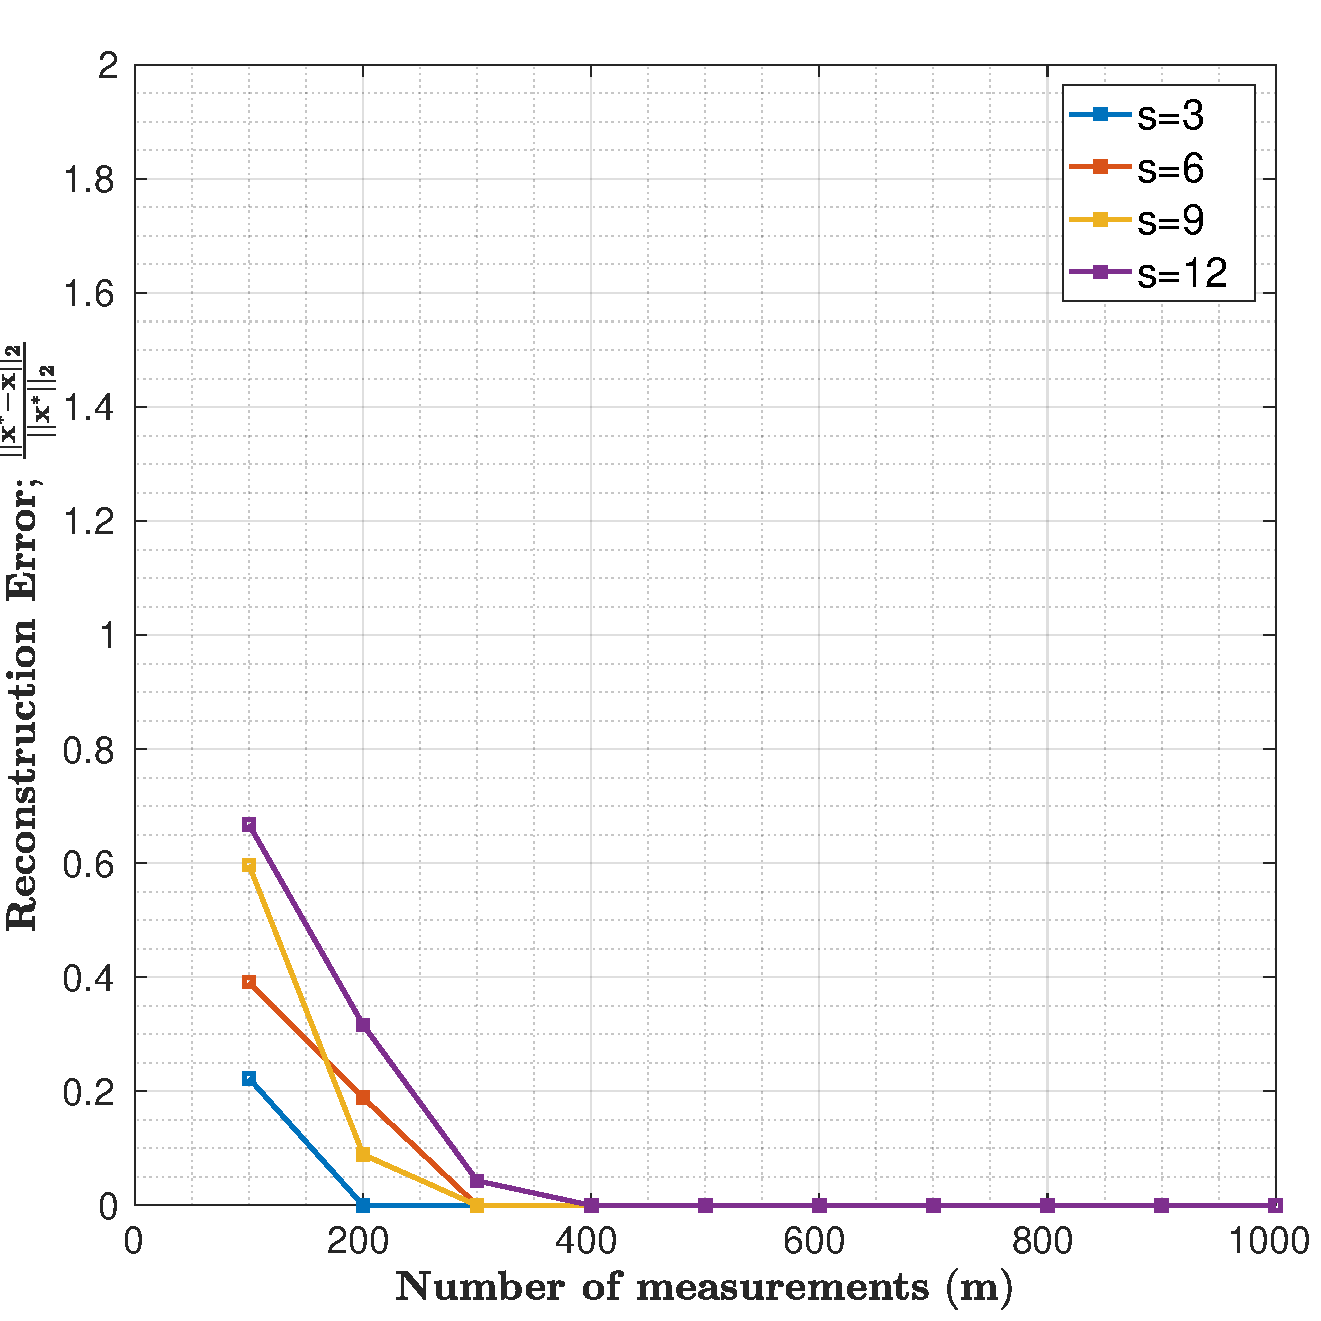
\includegraphics[width=0.9\linewidth]{./fig/rconst_rcm_amp_1_r_1_s_3_12_m_100_1000_justice-pursuit.pdf}
%	\end{center}
%	\caption{{Mean relative reconstruction error vs no. of measurements $(m)$ for MoRAM with $\norm{\mb{x^*}}_2=1,R=1,n=1000$.}}
%	\label{fig:plot-r-1}
%\end{figure}


%\begin{figure}[t]
%	\begin{center}
%		%\vspace{-0em}
%		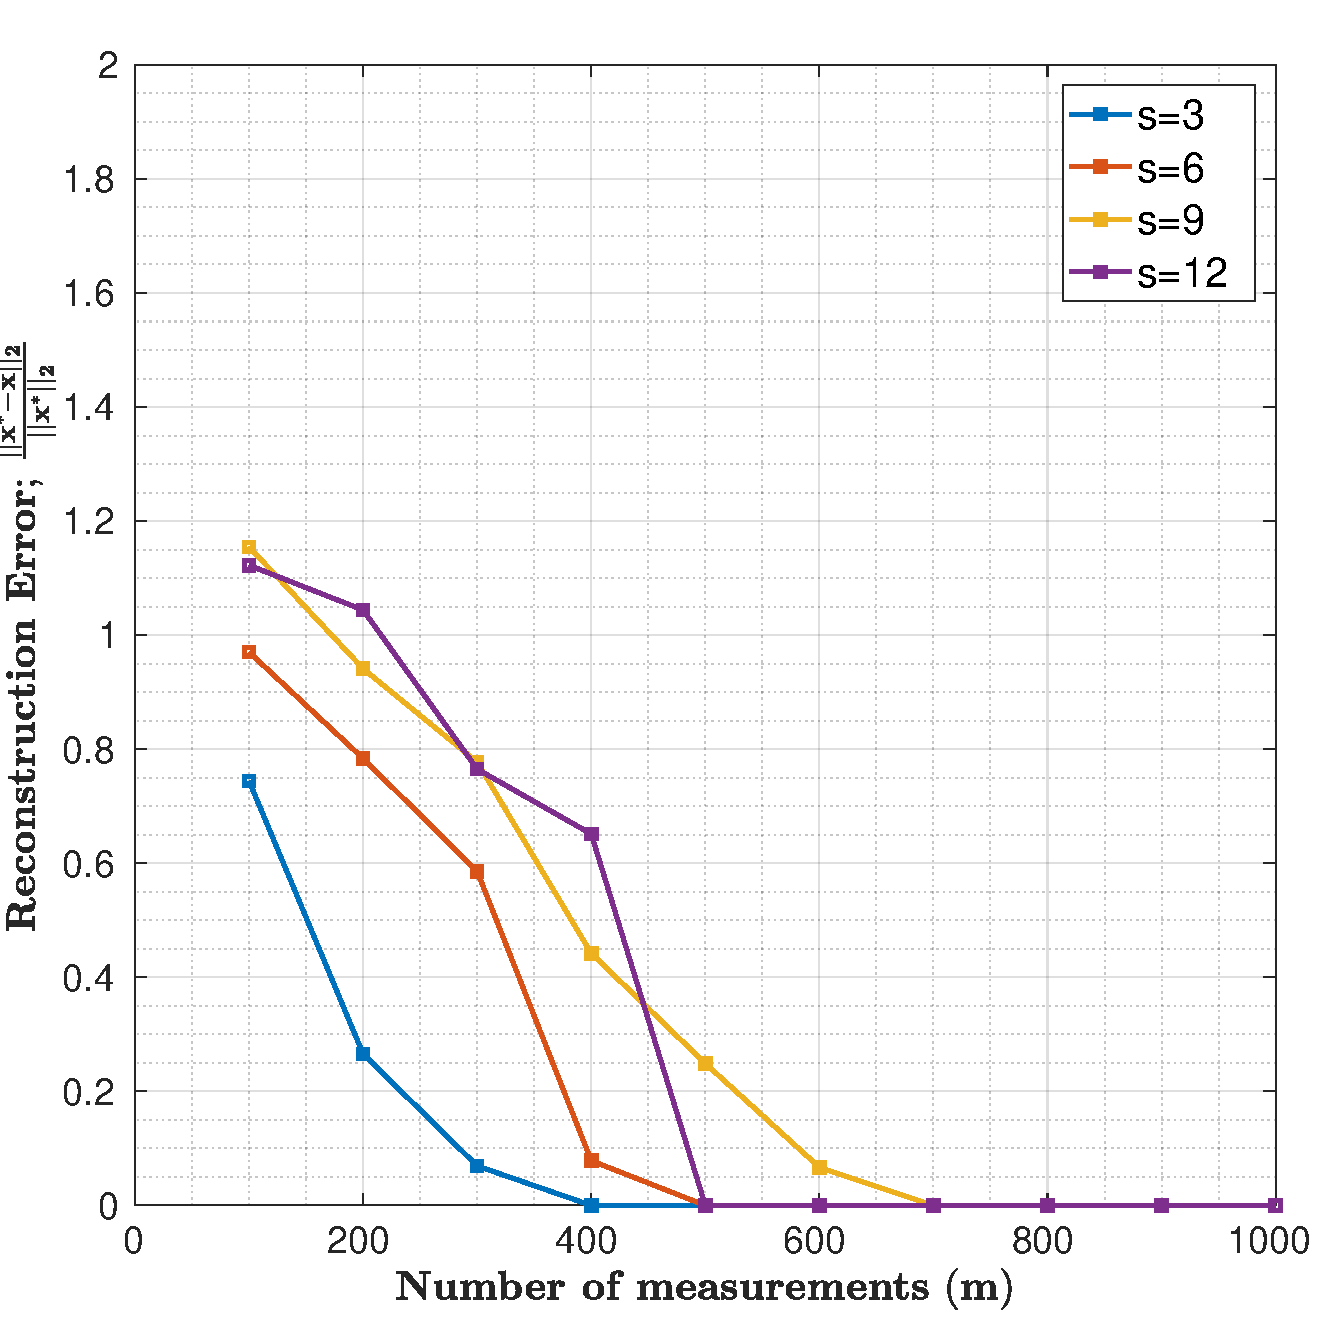
\includegraphics[width=0.9\linewidth]{./fig/rconst_rcm_amp_1_r_2_s_3_12_m_100_1000_justice-pursuit.pdf}
%	\end{center}
%	\caption{{Mean relative reconstruction error vs no. of measurements $(m)$ for MoRAM with $\norm{\mb{x^*}}_2=1,R=2,n=1000$.}}
%	\label{fig:plot-r-2}
%\end{figure}
%
%
%\begin{figure}[t]
%	\begin{center}
%		%\vspace{-0em}
%		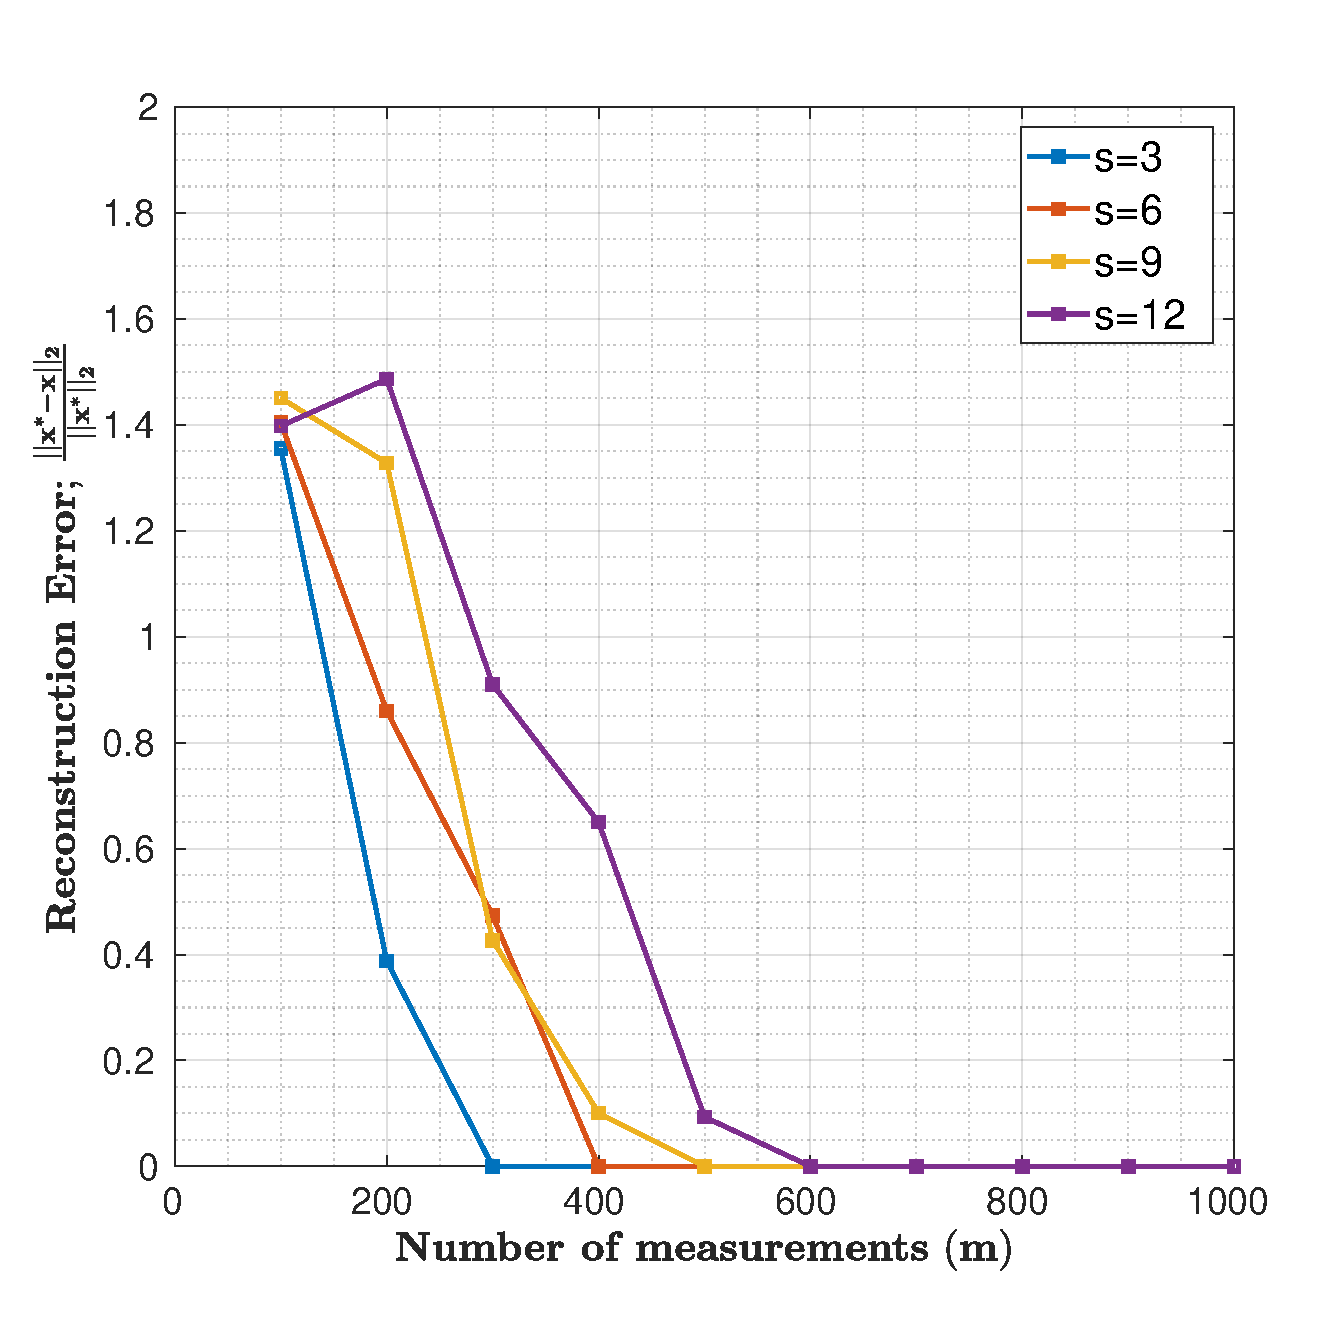
\includegraphics[width=0.9\linewidth]{./fig/rconst_rcm_amp_1_r_4_s_3_12_m_100_1000_justice-pursuit.pdf}
%	\end{center}
%	\caption{{Mean relative reconstruction error vs no. of measurements $(m)$ for MoRAM with $\norm{\mb{x^*}}_2=1,R=4,n=1000$.}}
%	\label{fig:plot-r-4}
%\end{figure}

%\begin{figure*}[!t]
%	\begin{center}
%	\begin{tabular}{ccc}
%		%\vspace{-0em}
%		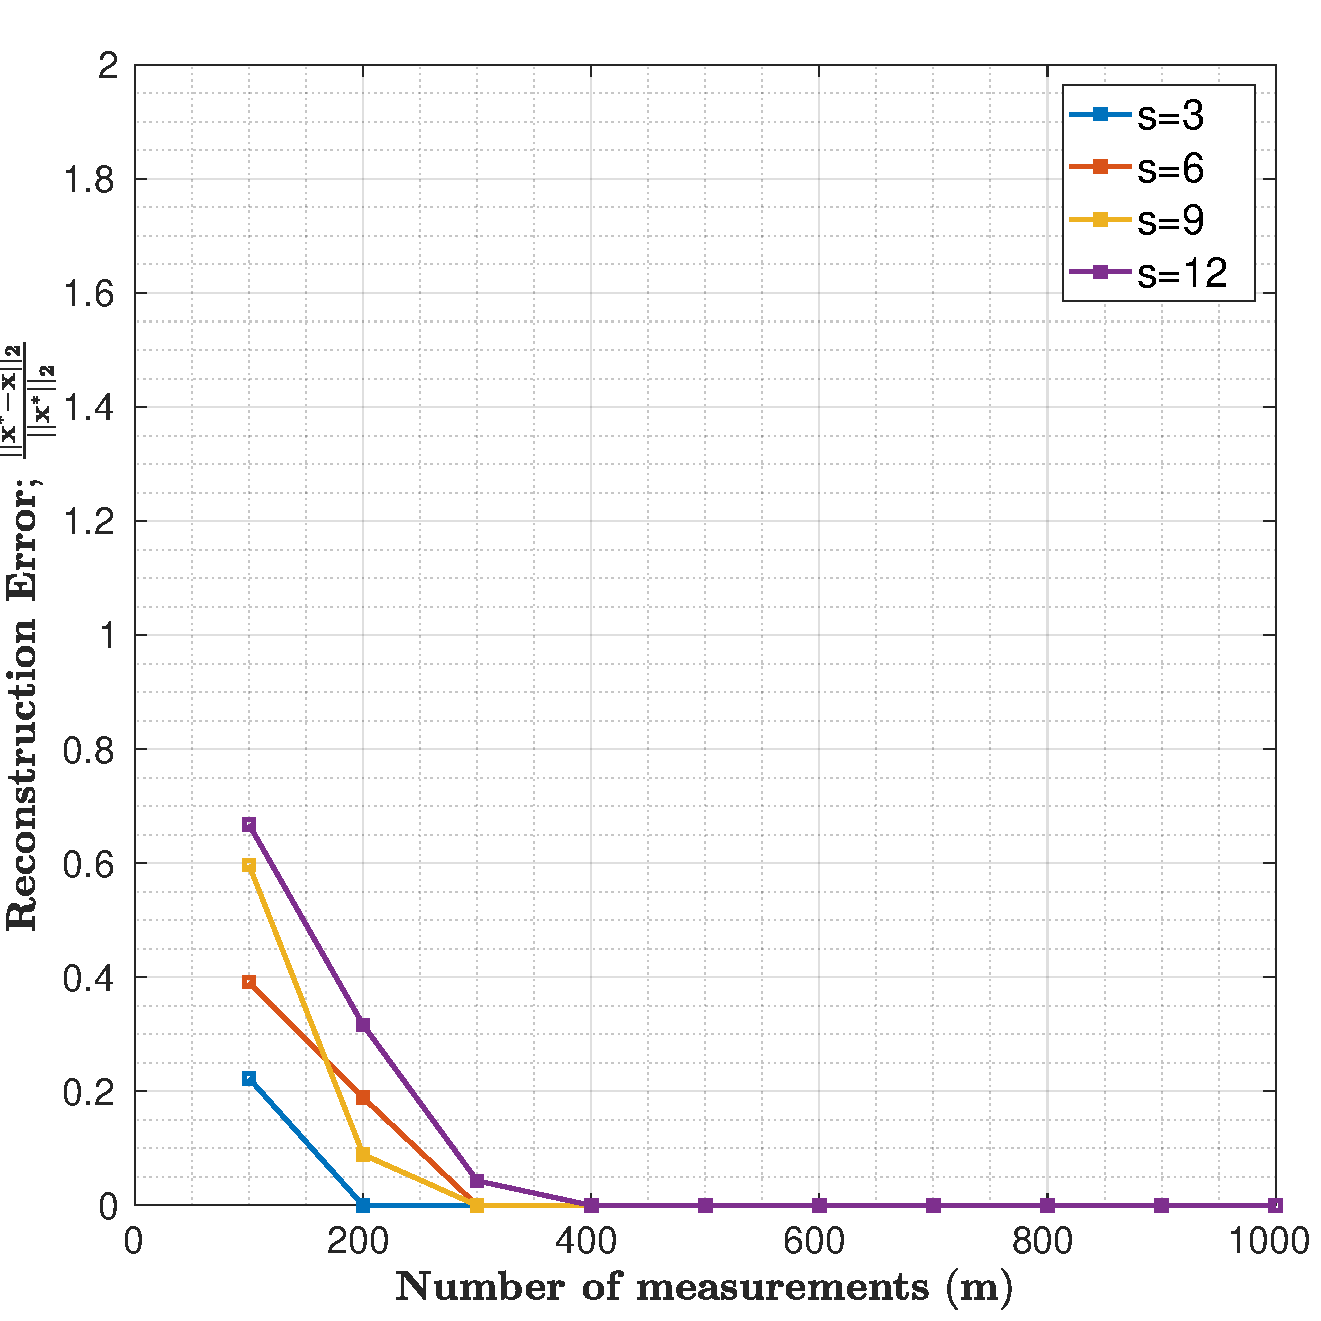
\includegraphics[width=0.3\textwidth]{./fig/rconst_rcm_amp_1_r_1_s_3_12_m_100_1000_justice-pursuit.pdf}
%	%\end{center}
%%	\caption{{Mean relative reconstruction error vs no. of measurements $(m)$ for MoRAM with $\norm{\mb{x^*}}_2=1,R=1,n=1000$.}}
%%	\label{fig:plot-r-1}
%%\end{figure}
%&
%
%%\begin{figure}[t]
%%	\begin{center}
%		%\vspace{-0em}
%		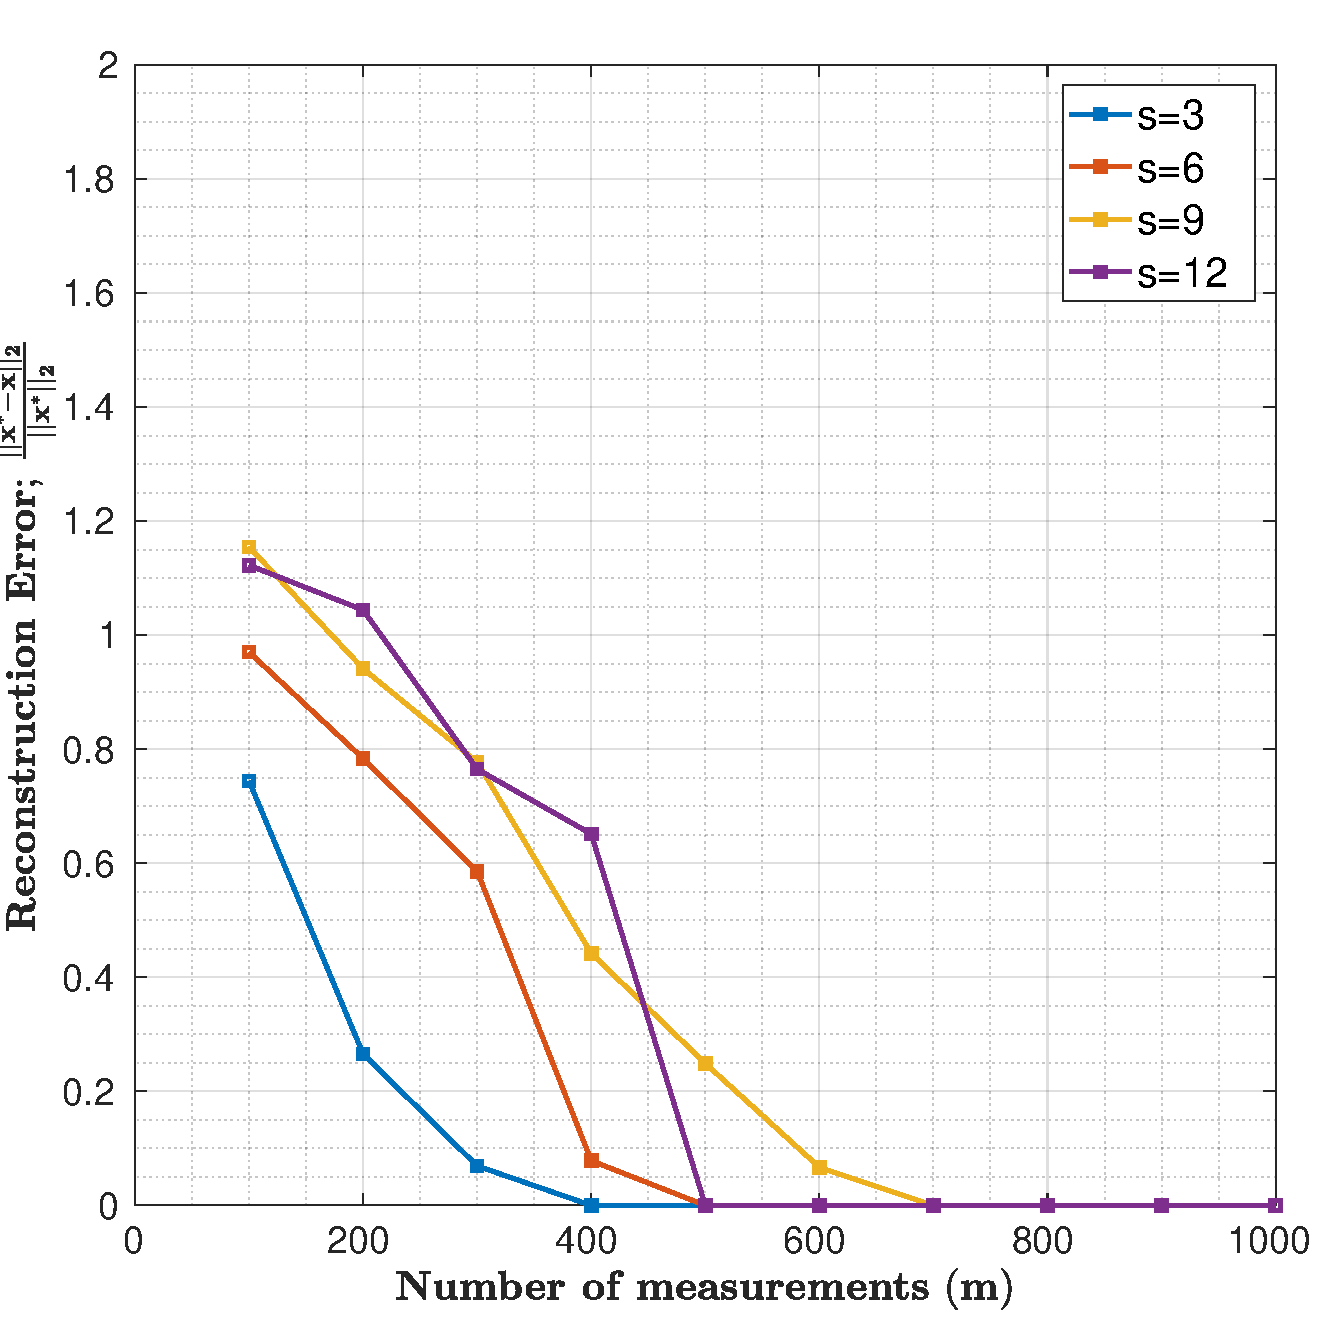
\includegraphics[width=0.3\textwidth]{./fig/rconst_rcm_amp_1_r_2_s_3_12_m_100_1000_justice-pursuit.pdf}
%%	\end{center}
%%	\caption{{Mean relative reconstruction error vs no. of measurements $(m)$ for MoRAM with $\norm{\mb{x^*}}_2=1,R=2,n=1000$.}}
%%	\label{fig:plot-r-2}
%%\end{figure}
%&
%
%%\begin{figure}[t]
%%	\begin{center}
%		%\vspace{-0em}
%		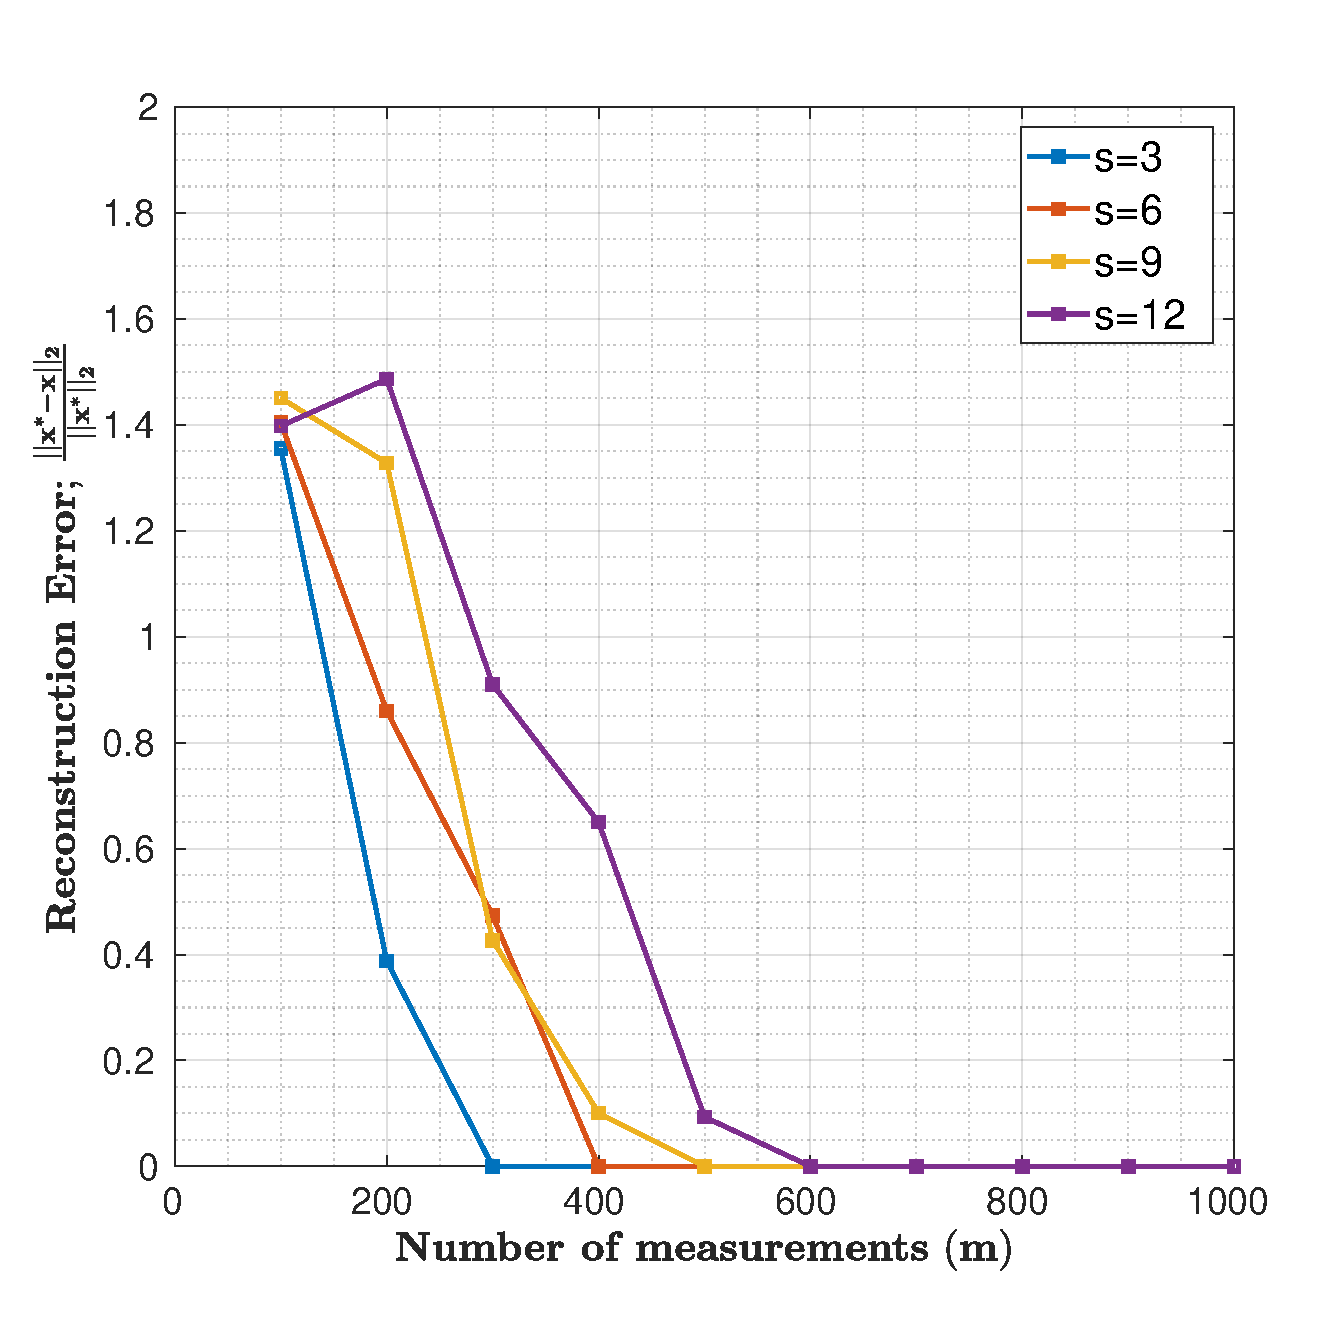
\includegraphics[width=0.3\textwidth]{./fig/rconst_rcm_amp_1_r_4_s_3_12_m_100_1000_justice-pursuit.pdf}
%\end{tabular}
%	\end{center}
%%	\caption{{Mean relative reconstruction error vs no. of measurements $(m)$ for MoRAM with $\norm{\mb{x^*}}_2=1,R=4,n=1000$.}}
%%	\label{fig:plot-r-4}
%\end{figure*}


%\begin{figure}[h]
%	\begin{center}
%		%\vspace{-0em}
%		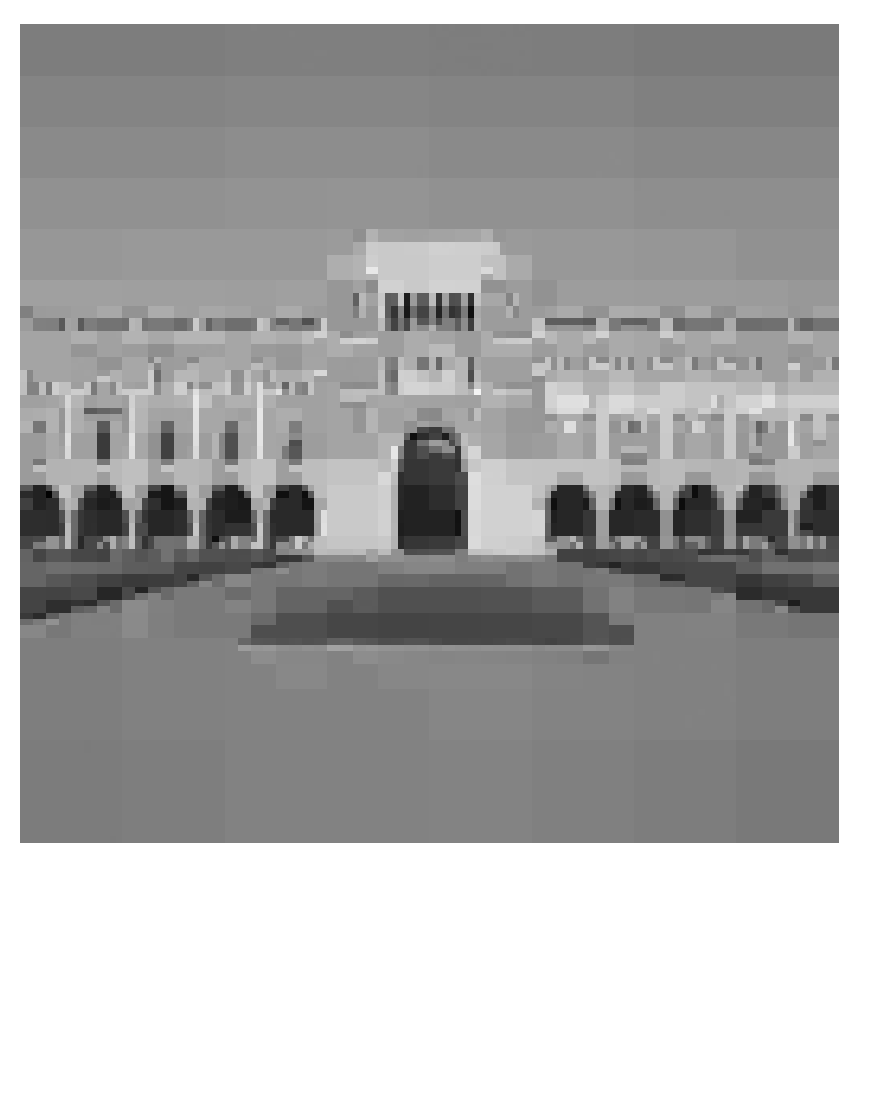
\includegraphics[width=0.9\linewidth]{./fig/reconst_lovett.pdf}
%	\end{center}
%	\caption{{Reconstruction using MoRAM}}
%	\label{fig:lovettreconst}
%\end{figure}
%\begin{figure}[!t]
%	\centering
%	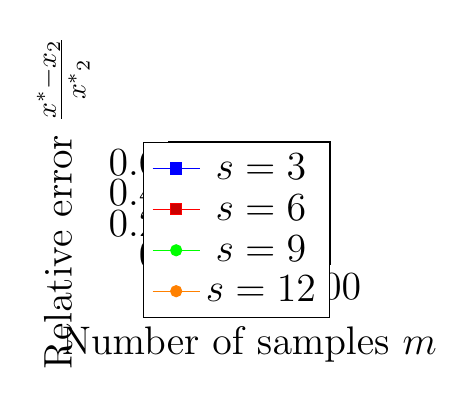
\begin{tikzpicture}
\begin{axis}
[width=0.3\textwidth,
xlabel= Number of samples $m$, 
ylabel= Relative error $\frac{\norm{\mb{x^*-x}}_2}{\norm{\mb{x^*}}_2}$,
grid style = dashed,
grid=both,
legend style=
{
at={(1,1), %for arxiv version
%at={(1.65,0.8),  %for NIPS version
anchor=top},
cells={align=center}, 
%legend columns=-1,
} 
]

\addplot[color=blue,mark=square*] plot coordinates {
	(100, 0.222952795500352)
	(200, 8.25E-05)
	(300, 6.48E-05)
	(400, 6.37E-05)
	(500, 7.91E-05)
 	(600, 6.45E-05)
	(700, 5.51E-05)
	(800, 4.77E-05)
	(900, 6.78E-05)
	(1000, 5.76E-05)
};
\addlegendentry{$s=3$};


\addplot plot coordinates {
(100,	0.391717206388554)
(200,	0.189009904901885)
(300,	8.75E-05)
(400,	6.63E-05)
(500,	7.39E-05)
(600,	6.96E-05)
(700,	5.79E-05)
(800,   6.41E-05)
(900,	8.06E-05)
(1000,	6.78E-05)
};

\addlegendentry{$s=6$};


\addplot[color=green,mark=*] plot coordinates {
(100,0.596874049564358)
(200,0.0893297570309944)
(300,0.0000961819292563893)
(400,0.0000965366166880477)
(500,0.0000950192717929039)
(600,0.0000992956375702069)
(700,0.0000835965044892149)
(800,0.0000675354618845817)
(900,0.0000811820156888768)
(1000,0.000064977150825922)
};
\addlegendentry{$s=9$};

\addplot[color=orange,mark=*] plot coordinates {
(100,0.667881390121055)
(200,0.316701449929789)
(300,0.0432277244535189)
(400,0.000108785027973407)
(500,0.0000962070190416804)
(600,0.0000899199807562489)
(700,0.000102447155819804)
(800,0.0000922462885218879)
(900,0.0000888147784526045)
(1000,0.0000753141220088111)

};
\addlegendentry{$s=12$};



%\legend{CoPRAM\\Block CoPRAM\\ThWF\\SPARTA\\}

\end{axis}
\end{tikzpicture}
%	\caption{\sl Mean relative reconstruction error vs no. of measurements $(m)$ for MoRAM with $\norm{\mb{x^*}}_2=1,R=1,n=1000$.} \label{fig:plot-r-1}
%\end{figure}
%
%\begin{figure}[!t]
%	\centering
%	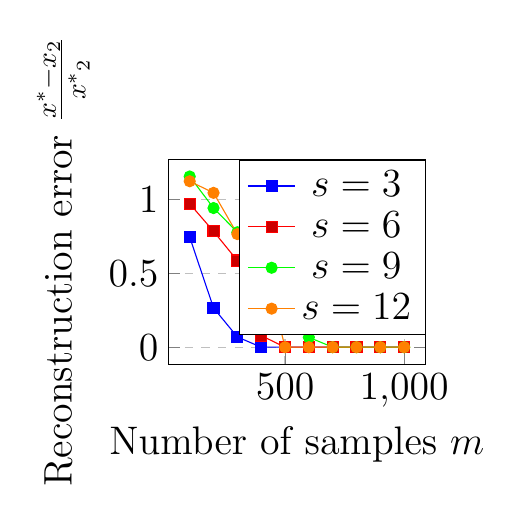
\begin{tikzpicture}
\begin{axis}
[width=0.4\textwidth,
xlabel= Number of samples $m$, 
ylabel= Reconstruction error $\frac{\norm{\mb{x^*-x}}_2}{\norm{\mb{x^*}}_2}$,
grid style = dashed,
grid=both,
legend style=
{
	at={(1,1), %for arxiv version
		%at={(1.65,0.8),  %for NIPS version
		anchor=top},
	cells={align=center}, 
	%legend columns=-1,
} 
]

\addplot[color=blue,mark=square*] plot coordinates {
	(100,0.74427083497336)
	(200,0.26556282505296)
	(300,0.0693282329160152)
	(400,0.0000759947449506268)
	(500,0.0000703837475666469)
	(600,0.0000522047439857151)
	(700,0.0000638145267540324)
	(800,0.000053588062967525)
	(900,0.0000341906002745844)
	(1000,0.0000649790103329161)
	
};
\addlegendentry{$s=3$};


\addplot plot coordinates {
	(100,0.970200248504512)
	(200,0.783733967580109)
	(300,0.585896829880407)
	(400,0.0785807046200051)
	(500,0.0000841836424731131)
	(600,0.0000758879406272977)
	(700,0.0000712248016620914)
	(800,0.0000609478657003822)
	(900,0.0000823001981803784)
	(1000,0.0000652284523240285)
	
};

\addlegendentry{$s=6$};


\addplot[color=green,mark=*] plot coordinates {
	(100,1.15475705568194)
	(200,0.941209335557007)
	(300,0.777520369268922)
	(400,0.442101179084315)
	(500,0.249049460556818)
	(600,0.066874088406845)
	(700,0.0000934401692366995)
	(800,0.0000832753637218933)
	(900,0.0000718321294789104)
	(1000,0.0000674942823198963)
	
};
\addlegendentry{$s=9$};

\addplot[color=orange,mark=*] plot coordinates {
	(100,1.12249994092088)
	(200,1.04403070665004)
	(300,0.76510361311149)
	(400,0.65138560583711)
	(500,0.000087283006450878)
	(600,0.000101093733403955)
	(700,0.0000771972799083333)
	(800,0.0000768498307046639)
	(900,0.0000962856213515402)
	(1000,0.0000790639986588349)
};
\addlegendentry{$s=12$};



%\legend{CoPRAM\\Block CoPRAM\\ThWF\\SPARTA\\}

\end{axis}
\end{tikzpicture}
%	\caption{\sl Mean relative reconstruction error vs no. of measurements $(m)$ for MoRAM with $\norm{\mb{x^*}}_2=1,R=2,n=1000$.} \label{fig:plot-r-2}
%\end{figure}
%
%\begin{figure}[!t]
%	\centering
%	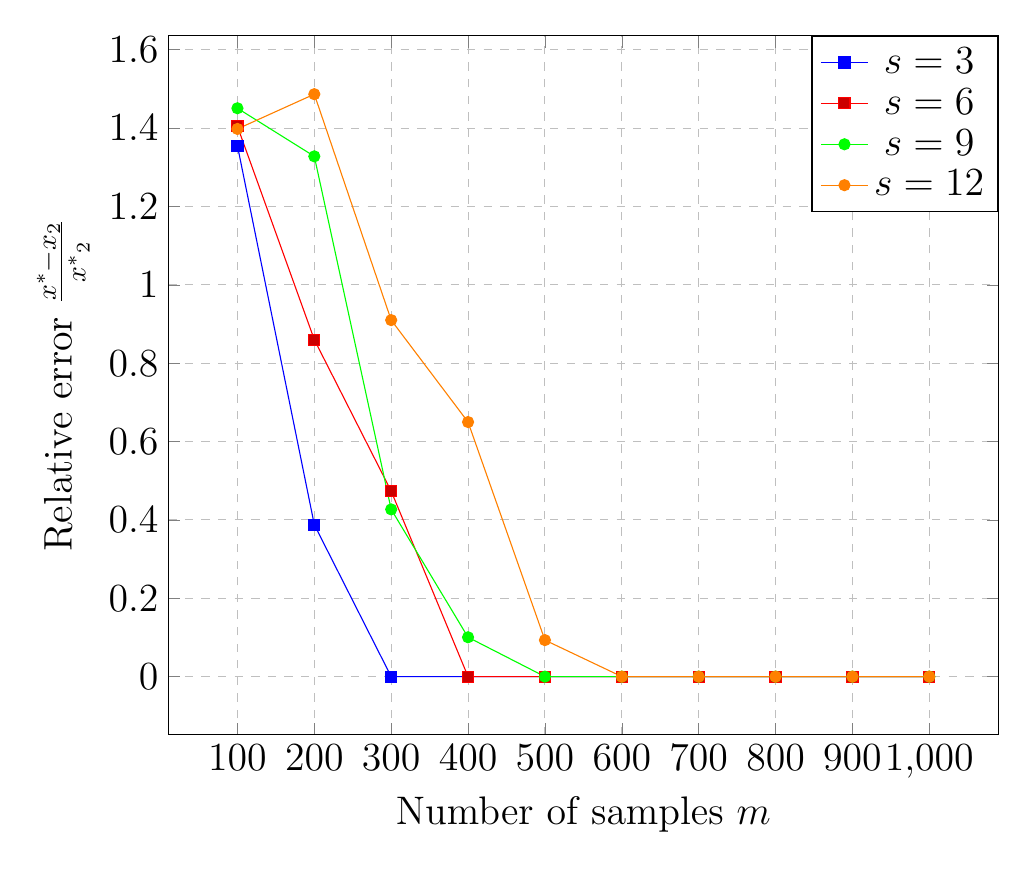
\begin{tikzpicture}
\tikzstyle{every node}=[font=\Large]
\begin{axis}
[width=\linewidth,
xlabel= Number of samples $m$, 
ylabel= Relative error $\frac{\norm{\mb{x^*-x}}_2}{\norm{\mb{x^*}}_2}$,
grid style = dashed,
grid=both,
legend style=
{
at={(1,1), %for arxiv version
%at={(1.65,0.8),  %for NIPS version
anchor=top},
cells={align=center}, 
%legend columns=-1,
} 
]

\addplot[color=blue,mark=square*] plot coordinates {
(100,1.35491249236152)
(200,0.387834861360979)
(300,0.0000838932462760031)
(400,0.0000796709195404289)
(500,0.0000699847485553827)
(600,0.0000654248964096406)
(700,0.0000556622044076941)
(800,0.0000577754338669424)
(900,0.0000476093461140991)
(1000,0.000050430624642886)

};
\addlegendentry{$s=3$};


\addplot plot coordinates {
(100,1.4044226284938)
(200,0.860030446367654)
(300,0.473492899335313)
(400,0.0000833934372627376)
(500,0.0000824008767554939)
(600,0.0000637716674864768)
(700,0.0000644672859553126)
(800,0.0000649831938234799)
(900,0.0000692018122982395)
(1000,0.0000633648746645319)

};

\addlegendentry{$s=6$};


\addplot[color=green,mark=*] plot coordinates {
(100,1.45063072923552)
(200,1.32791017206988)
(300,0.426899433442911)
(400,0.100521404653474)
(500,0.0000847861906819546)
(600,0.0000874052339854557)
(700,0.0000975048393826316)
(800,0.000072296472052776)
(900,0.0000706944130642887)
(1000,0.0000730819848601016)

};
\addlegendentry{$s=9$};

\addplot[color=orange,mark=*] plot coordinates {
(100,1.39786595436235)
(200,1.48655013005159)
(300,0.909955665520478)
(400,0.649802110302209)
(500,0.0932660496014009)
(600,0.0000913091790977068)
(700,0.000104507094662964)
(800,0.0000965628384101342)
(900,0.0000934605996504098)
(1000,0.0000841210242777489)	
};
\addlegendentry{$s=12$};



%\legend{CoPRAM\\Block CoPRAM\\ThWF\\SPARTA\\}

\end{axis}
\end{tikzpicture}
%	\caption{\sl Mean relative reconstruction error vs no. of measurements $(m)$ for MoRAM with $\norm{\mb{x^*}}_2=1,R=4,n=1000$.} \label{fig:plot-r-4}
%\end{figure}

